\documentclass[twoside]{book}

% Packages required by doxygen
\usepackage{fixltx2e}
\usepackage{calc}
\usepackage{doxygen}
\usepackage[export]{adjustbox} % also loads graphicx
\usepackage{graphicx}
\usepackage[utf8]{inputenc}
\usepackage{makeidx}
\usepackage{multicol}
\usepackage{multirow}
\PassOptionsToPackage{warn}{textcomp}
\usepackage{textcomp}
\usepackage[nointegrals]{wasysym}
\usepackage[table]{xcolor}

% Font selection
\usepackage[T1]{fontenc}
\usepackage[scaled=.90]{helvet}
\usepackage{courier}
\usepackage{amssymb}
\usepackage{sectsty}
\renewcommand{\familydefault}{\sfdefault}
\allsectionsfont{%
  \fontseries{bc}\selectfont%
  \color{darkgray}%
}
\renewcommand{\DoxyLabelFont}{%
  \fontseries{bc}\selectfont%
  \color{darkgray}%
}
\newcommand{\+}{\discretionary{\mbox{\scriptsize$\hookleftarrow$}}{}{}}

% Page & text layout
\usepackage{geometry}
\geometry{%
  a4paper,%
  top=2.5cm,%
  bottom=2.5cm,%
  left=2.5cm,%
  right=2.5cm%
}
\tolerance=750
\hfuzz=15pt
\hbadness=750
\setlength{\emergencystretch}{15pt}
\setlength{\parindent}{0cm}
\setlength{\parskip}{0.2cm}
\makeatletter
\renewcommand{\paragraph}{%
  \@startsection{paragraph}{4}{0ex}{-1.0ex}{1.0ex}{%
    \normalfont\normalsize\bfseries\SS@parafont%
  }%
}
\renewcommand{\subparagraph}{%
  \@startsection{subparagraph}{5}{0ex}{-1.0ex}{1.0ex}{%
    \normalfont\normalsize\bfseries\SS@subparafont%
  }%
}
\makeatother

% Headers & footers
\usepackage{fancyhdr}
\pagestyle{fancyplain}
\fancyhead[LE]{\fancyplain{}{\bfseries\thepage}}
\fancyhead[CE]{\fancyplain{}{}}
\fancyhead[RE]{\fancyplain{}{\bfseries\leftmark}}
\fancyhead[LO]{\fancyplain{}{\bfseries\rightmark}}
\fancyhead[CO]{\fancyplain{}{}}
\fancyhead[RO]{\fancyplain{}{\bfseries\thepage}}
\fancyfoot[LE]{\fancyplain{}{}}
\fancyfoot[CE]{\fancyplain{}{}}
\fancyfoot[RE]{\fancyplain{}{\bfseries\scriptsize Generated on Fri Apr 15 2016 09\+:44\+:14 for dev package by Doxygen }}
\fancyfoot[LO]{\fancyplain{}{\bfseries\scriptsize Generated on Fri Apr 15 2016 09\+:44\+:14 for dev package by Doxygen }}
\fancyfoot[CO]{\fancyplain{}{}}
\fancyfoot[RO]{\fancyplain{}{}}
\renewcommand{\footrulewidth}{0.4pt}
\renewcommand{\chaptermark}[1]{%
  \markboth{#1}{}%
}
\renewcommand{\sectionmark}[1]{%
  \markright{\thesection\ #1}%
}

% Indices & bibliography
\usepackage{natbib}
\usepackage[titles]{tocloft}
\setcounter{tocdepth}{3}
\setcounter{secnumdepth}{5}
\makeindex

% Hyperlinks (required, but should be loaded last)
\usepackage{ifpdf}
\ifpdf
  \usepackage[pdftex,pagebackref=true]{hyperref}
\else
  \usepackage[ps2pdf,pagebackref=true]{hyperref}
\fi
\hypersetup{%
  colorlinks=true,%
  linkcolor=blue,%
  citecolor=blue,%
  unicode%
}

% Custom commands
\newcommand{\clearemptydoublepage}{%
  \newpage{\pagestyle{empty}\cleardoublepage}%
}


%===== C O N T E N T S =====

\begin{document}

% Titlepage & ToC
\hypersetup{pageanchor=false,
             bookmarks=true,
             bookmarksnumbered=true,
             pdfencoding=unicode
            }
\pagenumbering{roman}
\begin{titlepage}
\vspace*{7cm}
\begin{center}%
{\Large dev package }\\
\vspace*{1cm}
{\large Generated by Doxygen 1.8.9.1}\\
\vspace*{0.5cm}
{\small Fri Apr 15 2016 09:44:14}\\
\end{center}
\end{titlepage}
\clearemptydoublepage
\tableofcontents
\clearemptydoublepage
\pagenumbering{arabic}
\hypersetup{pageanchor=true}

%--- Begin generated contents ---
\chapter{The Simple Package Management Tool}
\label{index}\hypertarget{index}{}\subsubsection*{N\+A\+M\+E}

devpkg -- Simple package management utility

\subsubsection*{S\+Y\+N\+O\+P\+S\+I\+S}


\begin{DoxyCode}
1 devpkg -I url | -L | -c configure-options | -m make-options | -i install-options | -d path | -S | -F url -B
       url
\end{DoxyCode}


\subsubsection*{D\+E\+S\+C\+R\+I\+P\+T\+I\+O\+N}

The {\bfseries devpkg} helps to {\itshape fetch}, {\itshape configure}, {\itshape build} and {\itshape install} packages in forms of {\ttfamily .tar.\+gz}, {\ttfamily .tar.\+bz2} and {\ttfamily .git} from internet.

\begin{quote}
You {\bfseries M\+U\+S\+T} use {\ttfamily devpkg -\/\+S} to initalize the data base first. \end{quote}


\subsubsection*{F\+U\+N\+C\+T\+I\+O\+N L\+E\+T\+T\+E\+R\+S}

{\ttfamily -\/\+I url}~\newline
 Install package from {\ttfamily url}, it will fetch, configure, make, install then clean up the fetch source code and other build-\/phase temporatily files

{\ttfamily -\/\+L}~\newline
 List urls of the installed packages if any

{\ttfamily -\/c configure-\/options}~\newline
 Setup the ./configure opruons

{\ttfamily -\/m make-\/options}~\newline
 Setup the make options

{\ttfamily -\/i install-\/options}~\newline
 Setup install options

{\ttfamily -\/d path}~\newline
 Install all urls in the \textquotesingle{}path\textquotesingle{} file, which contains url per line to install~\newline
 If You fetch depents file from internet, the file M\+U\+S\+T be {\ttfamily $\ast$.D\+E\+P\+E\+N\+D\+S}

{\ttfamily -\/\+S}~\newline
 Initalize the data base to store package urls which are installed

{\ttfamily -\/\+F url}~\newline
 Fetch the package source code from {\ttfamily url}

{\ttfamily -\/\+B url}~\newline
 Configure and Build the package of {\ttfamily url}

\subsubsection*{E\+N\+V\+I\+R\+O\+N\+M\+E\+N\+T}

The {\ttfamily devpkg -\/\+S} will creates a database file at {\ttfamily /usr/local/.devpkg/db}, which will record the installed package\textquotesingle{}s urls.~\newline
When {\ttfamily fetch}, {\ttfamily build} or {\ttfamily install} package, the package compressed source code is at /tmp/pkg-\/src.tar.\mbox{[}gz$\vert$bz2\mbox{]}, and the build-\/phase temporatily files is at /tmp/pkg-\/build. After install the package, those two directorues will be cleanup.

\subsubsection*{E\+X\+A\+M\+P\+L\+E}

Fetch package source from url\+: {\ttfamily foo.\+bar}. 
\begin{DoxyCode}
1 devpkg -F foo.bar
\end{DoxyCode}


Install package from url\+: {\ttfamily foo.\+bar} using configure options\+:{\ttfamily c-\/opts}, make options\+: {\ttfamily m-\/opts}, install options\+: {\ttfamily i-\/opts}. 
\begin{DoxyCode}
1 devpkg -c c-opts -m m-opts -i i-opts -I foo.bar
\end{DoxyCode}


List package we have installed if any. 
\begin{DoxyCode}
1 devpkg -L
\end{DoxyCode}


\subsubsection*{B\+U\+G\+S}

\subsubsection*{T\+O\+D\+O}


\begin{DoxyItemize}
\item \mbox{[} \mbox{]} Some packages need ./autoconfig, but we don\textquotesingle{}t implement it.
\item \mbox{[} \mbox{]} {\ttfamily devpkg -\/d xxx.\+D\+E\+P\+E\+N\+D\+S} can\textquotesingle{}t input configure options, make options, and install options.
\item \mbox{[} \mbox{]} Don\textquotesingle{}t check the integrity(ex. md5). 
\end{DoxyItemize}
\chapter{Class Index}
\section{Class List}
Here are the classes, structs, unions and interfaces with brief descriptions\+:\begin{DoxyCompactList}
\item\contentsline{section}{\hyperlink{structbStream}{b\+Stream} }{\pageref{structbStream}}{}
\item\contentsline{section}{\hyperlink{structbstrList}{bstr\+List} }{\pageref{structbstrList}}{}
\item\contentsline{section}{\hyperlink{structcharField}{char\+Field} }{\pageref{structcharField}}{}
\item\contentsline{section}{\hyperlink{structgenBstrList}{gen\+Bstr\+List} }{\pageref{structgenBstrList}}{}
\item\contentsline{section}{\hyperlink{structShell}{Shell} }{\pageref{structShell}}{}
\item\contentsline{section}{\hyperlink{structtagbstring}{tagbstring} }{\pageref{structtagbstring}}{}
\end{DoxyCompactList}

\chapter{File Index}
\section{File List}
Here is a list of all documented files with brief descriptions\+:\begin{DoxyCompactList}
\item\contentsline{section}{{\bfseries bstrlib.\+h} }{\pageref{bstrlib_8h}}{}
\item\contentsline{section}{\hyperlink{commands_8c}{commands.\+c} \\*Commands }{\pageref{commands_8c}}{}
\item\contentsline{section}{\hyperlink{commands_8h}{commands.\+h} \\*Commands }{\pageref{commands_8h}}{}
\item\contentsline{section}{\hyperlink{db_8c}{db.\+c} \\*Simple data base }{\pageref{db_8c}}{}
\item\contentsline{section}{\hyperlink{db_8h}{db.\+h} \\*Database }{\pageref{db_8h}}{}
\item\contentsline{section}{\hyperlink{devpkg_8c}{devpkg.\+c} \\*Packages manage main function }{\pageref{devpkg_8c}}{}
\item\contentsline{section}{\hyperlink{shell_8c}{shell.\+c} \\*\hyperlink{structShell}{Shell} }{\pageref{shell_8c}}{}
\item\contentsline{section}{\hyperlink{shell_8h}{shell.\+h} \\*\hyperlink{structShell}{Shell} header }{\pageref{shell_8h}}{}
\end{DoxyCompactList}

\chapter{Class Documentation}
\hypertarget{structbStream}{}\section{b\+Stream Struct Reference}
\label{structbStream}\index{b\+Stream@{b\+Stream}}


Collaboration diagram for b\+Stream\+:\nopagebreak
\begin{figure}[H]
\begin{center}
\leavevmode
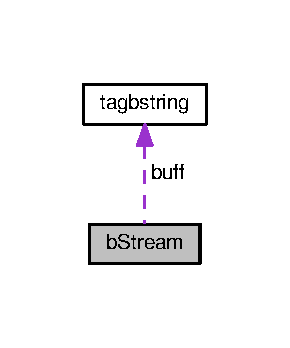
\includegraphics[width=139pt]{structbStream__coll__graph}
\end{center}
\end{figure}
\subsection*{Public Attributes}
\begin{DoxyCompactItemize}
\item 
\hypertarget{structbStream_aba3294390fa40724b5762adf073c1b86}{}\hyperlink{structtagbstring}{bstring} {\bfseries buff}\label{structbStream_aba3294390fa40724b5762adf073c1b86}

\item 
\hypertarget{structbStream_a43b389e3157aea7f84ba553ad7b24e3e}{}void $\ast$ {\bfseries parm}\label{structbStream_a43b389e3157aea7f84ba553ad7b24e3e}

\item 
\hypertarget{structbStream_a4279a6d91f9df1f4f3dc157d18479491}{}b\+Nread {\bfseries read\+Fn\+Ptr}\label{structbStream_a4279a6d91f9df1f4f3dc157d18479491}

\item 
\hypertarget{structbStream_a7d014819731e1d0415ba4ff92e80ffda}{}int {\bfseries is\+E\+O\+F}\label{structbStream_a7d014819731e1d0415ba4ff92e80ffda}

\item 
\hypertarget{structbStream_a952ac9807d96d9d1dc510ed4bdc8b257}{}int {\bfseries max\+Buff\+Sz}\label{structbStream_a952ac9807d96d9d1dc510ed4bdc8b257}

\end{DoxyCompactItemize}


The documentation for this struct was generated from the following file\+:\begin{DoxyCompactItemize}
\item 
bstrlib.\+c\end{DoxyCompactItemize}

\hypertarget{structbstrList}{}\section{bstr\+List Struct Reference}
\label{structbstrList}\index{bstr\+List@{bstr\+List}}


Collaboration diagram for bstr\+List\+:\nopagebreak
\begin{figure}[H]
\begin{center}
\leavevmode
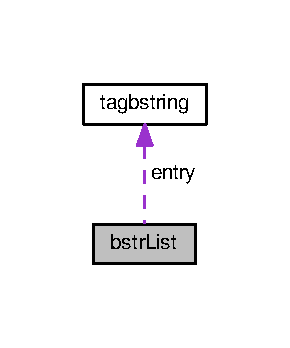
\includegraphics[width=139pt]{structbstrList__coll__graph}
\end{center}
\end{figure}
\subsection*{Public Attributes}
\begin{DoxyCompactItemize}
\item 
\hypertarget{structbstrList_a23465fcc1c43891c136fead866a30a0e}{}int {\bfseries qty}\label{structbstrList_a23465fcc1c43891c136fead866a30a0e}

\item 
\hypertarget{structbstrList_a27cec944f3421d6faaaaca651391eeb3}{}int {\bfseries mlen}\label{structbstrList_a27cec944f3421d6faaaaca651391eeb3}

\item 
\hypertarget{structbstrList_adab677d642e53205ebee8fd432977afc}{}\hyperlink{structtagbstring}{bstring} $\ast$ {\bfseries entry}\label{structbstrList_adab677d642e53205ebee8fd432977afc}

\end{DoxyCompactItemize}


The documentation for this struct was generated from the following file\+:\begin{DoxyCompactItemize}
\item 
bstrlib.\+h\end{DoxyCompactItemize}

\hypertarget{structcharField}{}\section{char\+Field Struct Reference}
\label{structcharField}\index{char\+Field@{char\+Field}}
\subsection*{Public Attributes}
\begin{DoxyCompactItemize}
\item 
\hypertarget{structcharField_a8f9248fefe062f32178d961d330454a1}{}L\+O\+N\+G\+\_\+\+T\+Y\+P\+E {\bfseries content} \mbox{[}C\+F\+C\+L\+E\+N\mbox{]}\label{structcharField_a8f9248fefe062f32178d961d330454a1}

\end{DoxyCompactItemize}


The documentation for this struct was generated from the following file\+:\begin{DoxyCompactItemize}
\item 
bstrlib.\+c\end{DoxyCompactItemize}

\hypertarget{structgenBstrList}{}\section{gen\+Bstr\+List Struct Reference}
\label{structgenBstrList}\index{gen\+Bstr\+List@{gen\+Bstr\+List}}


Collaboration diagram for gen\+Bstr\+List\+:\nopagebreak
\begin{figure}[H]
\begin{center}
\leavevmode
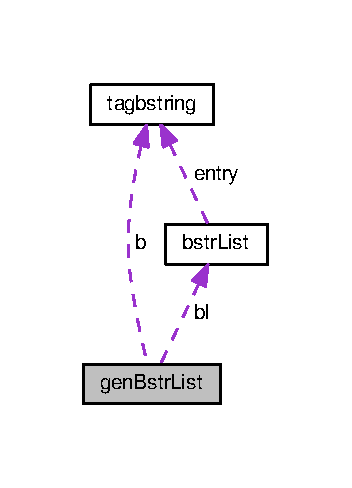
\includegraphics[width=169pt]{structgenBstrList__coll__graph}
\end{center}
\end{figure}
\subsection*{Public Attributes}
\begin{DoxyCompactItemize}
\item 
\hypertarget{structgenBstrList_afbc60fff27346f61f706e48aa9143cb2}{}\hyperlink{structtagbstring}{bstring} {\bfseries b}\label{structgenBstrList_afbc60fff27346f61f706e48aa9143cb2}

\item 
\hypertarget{structgenBstrList_abf9382d773a085b9015807e24ac8fbda}{}struct \hyperlink{structbstrList}{bstr\+List} $\ast$ {\bfseries bl}\label{structgenBstrList_abf9382d773a085b9015807e24ac8fbda}

\end{DoxyCompactItemize}


The documentation for this struct was generated from the following file\+:\begin{DoxyCompactItemize}
\item 
bstrlib.\+c\end{DoxyCompactItemize}

\hypertarget{structShell}{}\section{Shell Struct Reference}
\label{structShell}\index{Shell@{Shell}}
\subsection*{Public Attributes}
\begin{DoxyCompactItemize}
\item 
\hypertarget{structShell_af7f22d5f2b77da8d116c3c56799da8df}{}const char $\ast$ {\bfseries dir}\label{structShell_af7f22d5f2b77da8d116c3c56799da8df}

\item 
\hypertarget{structShell_aa383471cfa47390f167c9ccf20f96b1b}{}const char $\ast$ {\bfseries exe}\label{structShell_aa383471cfa47390f167c9ccf20f96b1b}

\item 
\hypertarget{structShell_ac69162f44ce6c9a5b1e942d59a0f564e}{}apr\+\_\+procattr\+\_\+t $\ast$ {\bfseries attr}\label{structShell_ac69162f44ce6c9a5b1e942d59a0f564e}

\item 
\hypertarget{structShell_ab344de6664e18cea93fac216148cda0e}{}apr\+\_\+proc\+\_\+t {\bfseries proc}\label{structShell_ab344de6664e18cea93fac216148cda0e}

\item 
\hypertarget{structShell_a4d87736ab735660ffdc6addc55cda406}{}apr\+\_\+exit\+\_\+why\+\_\+e {\bfseries exit\+\_\+why}\label{structShell_a4d87736ab735660ffdc6addc55cda406}

\item 
\hypertarget{structShell_a6d3a37fb42f08d96c562d7d05eacd293}{}int {\bfseries exit\+\_\+code}\label{structShell_a6d3a37fb42f08d96c562d7d05eacd293}

\item 
\hypertarget{structShell_a5c11ff22f0e7d22527ce3f40812adb2c}{}const char $\ast$ {\bfseries args} \mbox{[}M\+A\+X\+\_\+\+C\+O\+M\+M\+A\+N\+D\+\_\+\+A\+R\+G\+S\mbox{]}\label{structShell_a5c11ff22f0e7d22527ce3f40812adb2c}

\item 
\hypertarget{structShell_aa69f8cf1e84550e2aab58f34db08f4db}{}int {\bfseries need\+\_\+replace\+\_\+args\+\_\+count}\label{structShell_aa69f8cf1e84550e2aab58f34db08f4db}

\end{DoxyCompactItemize}


The documentation for this struct was generated from the following file\+:\begin{DoxyCompactItemize}
\item 
\hyperlink{shell_8h}{shell.\+h}\end{DoxyCompactItemize}

\hypertarget{structtagbstring}{}\section{tagbstring Struct Reference}
\label{structtagbstring}\index{tagbstring@{tagbstring}}
\subsection*{Public Attributes}
\begin{DoxyCompactItemize}
\item 
\hypertarget{structtagbstring_abf47839da62089f74883d8324f5ef539}{}int {\bfseries mlen}\label{structtagbstring_abf47839da62089f74883d8324f5ef539}

\item 
\hypertarget{structtagbstring_af9a7862da5259ad58776f27cbab88180}{}int {\bfseries slen}\label{structtagbstring_af9a7862da5259ad58776f27cbab88180}

\item 
\hypertarget{structtagbstring_aeacc0105c2eed78dcc0647f89898821f}{}unsigned char $\ast$ {\bfseries data}\label{structtagbstring_aeacc0105c2eed78dcc0647f89898821f}

\end{DoxyCompactItemize}


The documentation for this struct was generated from the following file\+:\begin{DoxyCompactItemize}
\item 
bstrlib.\+h\end{DoxyCompactItemize}

\chapter{File Documentation}
\hypertarget{commands_8c}{}\section{commands.\+c File Reference}
\label{commands_8c}\index{commands.\+c@{commands.\+c}}


commands  


{\ttfamily \#include $<$netdb.\+h$>$}\\*
{\ttfamily \#include $<$apr\+\_\+uri.\+h$>$}\\*
{\ttfamily \#include $<$apr\+\_\+fnmatch.\+h$>$}\\*
{\ttfamily \#include $<$unistd.\+h$>$}\\*
{\ttfamily \#include \char`\"{}commands.\+h\char`\"{}}\\*
{\ttfamily \#include \char`\"{}../../common/include/dbg.\+h\char`\"{}}\\*
{\ttfamily \#include \char`\"{}bstrlib.\+h\char`\"{}}\\*
{\ttfamily \#include \char`\"{}db.\+h\char`\"{}}\\*
{\ttfamily \#include \char`\"{}shell.\+h\char`\"{}}\\*
Include dependency graph for commands.\+c\+:\nopagebreak
\begin{figure}[H]
\begin{center}
\leavevmode
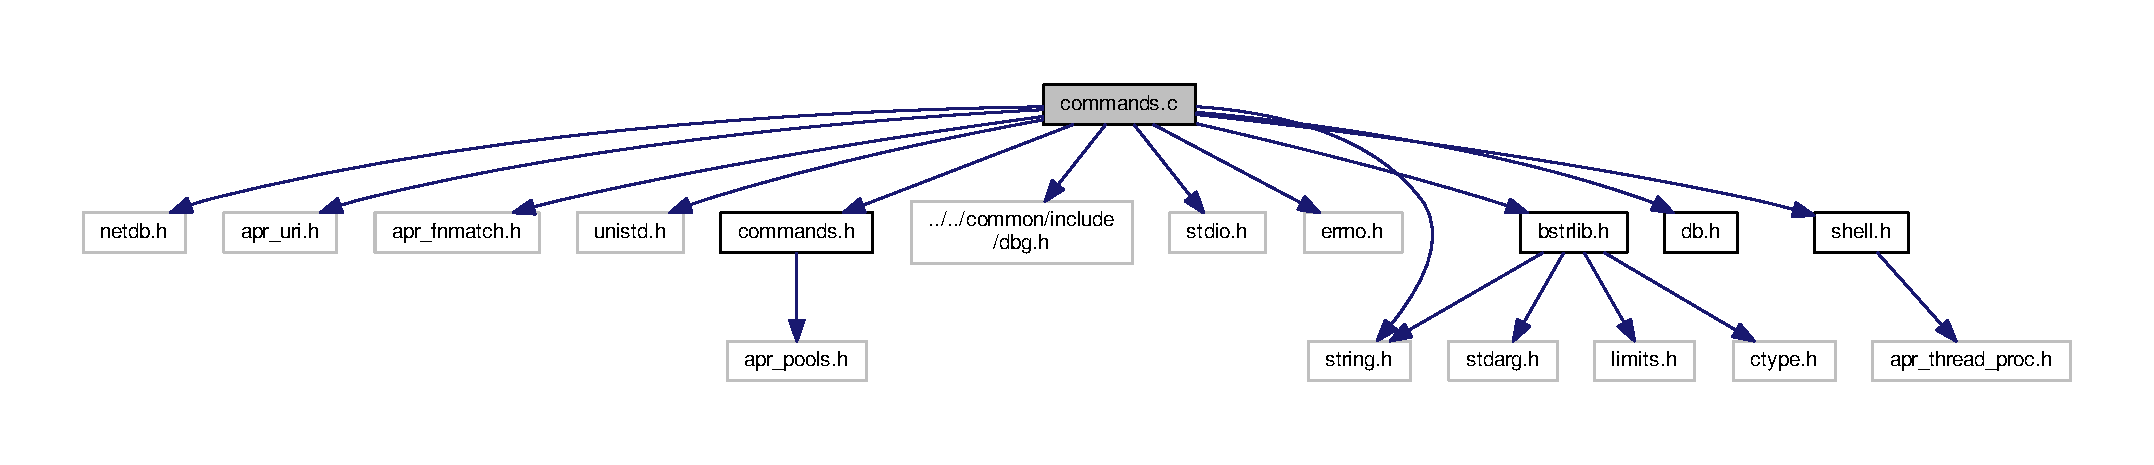
\includegraphics[width=350pt]{commands_8c__incl}
\end{center}
\end{figure}
\subsection*{Functions}
\begin{DoxyCompactItemize}
\item 
int \hyperlink{commands_8c_a8f5695cbe4457871b9ac8a7f686e93e9}{Command\+\_\+depends} (apr\+\_\+pool\+\_\+t $\ast$p, const char $\ast$path)
\begin{DoxyCompactList}\small\item\em install all depends package for path \end{DoxyCompactList}\item 
int \hyperlink{commands_8c_affbc6091a8bd093b418d1701bc2f7307}{Command\+\_\+fetch} (apr\+\_\+pool\+\_\+t $\ast$p, const char $\ast$url, int fetch\+\_\+only)
\begin{DoxyCompactList}\small\item\em fetch package from url \end{DoxyCompactList}\item 
int \hyperlink{commands_8c_a6910667dba531ef95fc0a445bdbf0141}{Command\+\_\+build} (apr\+\_\+pool\+\_\+t $\ast$p, const char $\ast$url, const char $\ast$configure\+\_\+opts, const char $\ast$make\+\_\+opts, const char $\ast$install\+\_\+opts)
\begin{DoxyCompactList}\small\item\em build package from url \end{DoxyCompactList}\item 
int \hyperlink{commands_8c_af384b213993ba94ca4f7e0492a544135}{Command\+\_\+install} (apr\+\_\+pool\+\_\+t $\ast$p, const char $\ast$url, const char $\ast$configure\+\_\+opts, const char $\ast$make\+\_\+opts, const char $\ast$install\+\_\+opts)
\begin{DoxyCompactList}\small\item\em Install package command. \end{DoxyCompactList}\end{DoxyCompactItemize}


\subsection{Detailed Description}
commands 

\begin{DoxyAuthor}{Author}
peter liu \href{mailto:peter.liu.work@gmail.com.tw}{\tt peter.\+liu.\+work@gmail.\+com.\+tw} 
\end{DoxyAuthor}
\begin{DoxyVersion}{Version}
0.\+0 
\end{DoxyVersion}
\begin{DoxyDate}{Date}
2016-\/04-\/13 
\end{DoxyDate}


\subsection{Function Documentation}
\hypertarget{commands_8c_a6910667dba531ef95fc0a445bdbf0141}{}\index{commands.\+c@{commands.\+c}!Command\+\_\+build@{Command\+\_\+build}}
\index{Command\+\_\+build@{Command\+\_\+build}!commands.\+c@{commands.\+c}}
\subsubsection[{Command\+\_\+build}]{\setlength{\rightskip}{0pt plus 5cm}int Command\+\_\+build (
\begin{DoxyParamCaption}
\item[{apr\+\_\+pool\+\_\+t $\ast$}]{p, }
\item[{const char $\ast$}]{url, }
\item[{const char $\ast$}]{configure\+\_\+opts, }
\item[{const char $\ast$}]{make\+\_\+opts, }
\item[{const char $\ast$}]{install\+\_\+opts}
\end{DoxyParamCaption}
)}\label{commands_8c_a6910667dba531ef95fc0a445bdbf0141}


build package from url 


\begin{DoxyParams}{Parameters}
{\em p} & A\+P\+R pool \\
\hline
{\em url} & url to build \\
\hline
{\em configure\+\_\+opts} & configure options \\
\hline
{\em make\+\_\+opts} & make options \\
\hline
{\em install\+\_\+opts} & install options\\
\hline
\end{DoxyParams}
\begin{DoxyReturn}{Returns}
{\bfseries 0}\+: build, make, install, cleanup, and database update successfully ~\newline
{\bfseries -\/1}\+: otherwise 
\end{DoxyReturn}
\hypertarget{commands_8c_a8f5695cbe4457871b9ac8a7f686e93e9}{}\index{commands.\+c@{commands.\+c}!Command\+\_\+depends@{Command\+\_\+depends}}
\index{Command\+\_\+depends@{Command\+\_\+depends}!commands.\+c@{commands.\+c}}
\subsubsection[{Command\+\_\+depends}]{\setlength{\rightskip}{0pt plus 5cm}int Command\+\_\+depends (
\begin{DoxyParamCaption}
\item[{apr\+\_\+pool\+\_\+t $\ast$}]{p, }
\item[{const char $\ast$}]{path}
\end{DoxyParamCaption}
)}\label{commands_8c_a8f5695cbe4457871b9ac8a7f686e93e9}


install all depends package for path 


\begin{DoxyParams}{Parameters}
{\em p} & A\+P\+R pool \\
\hline
{\em path} & depends file path which contains a url per line\\
\hline
\end{DoxyParams}
\begin{DoxyReturn}{Returns}
{\bfseries 0}\+: All dependes are installed successfully ~\newline
{\bfseries -\/1}\+: Otherwise 
\end{DoxyReturn}
\hypertarget{commands_8c_affbc6091a8bd093b418d1701bc2f7307}{}\index{commands.\+c@{commands.\+c}!Command\+\_\+fetch@{Command\+\_\+fetch}}
\index{Command\+\_\+fetch@{Command\+\_\+fetch}!commands.\+c@{commands.\+c}}
\subsubsection[{Command\+\_\+fetch}]{\setlength{\rightskip}{0pt plus 5cm}int Command\+\_\+fetch (
\begin{DoxyParamCaption}
\item[{apr\+\_\+pool\+\_\+t $\ast$}]{p, }
\item[{const char $\ast$}]{url, }
\item[{int}]{fetch\+\_\+only}
\end{DoxyParamCaption}
)}\label{commands_8c_affbc6091a8bd093b418d1701bc2f7307}


fetch package from url 


\begin{DoxyParams}{Parameters}
{\em p} & A\+P\+R pool \\
\hline
{\em url} & url to fetch \\
\hline
{\em fetch\+\_\+only} & fetch only\\
\hline
\end{DoxyParams}
\begin{DoxyReturn}{Returns}
{\bfseries 1}\+: fetch success, need to build \& install ~\newline
{\bfseries 0}\+: fetch success, nothing to do ~\newline
{\bfseries -\/1}\+: fetch error 
\end{DoxyReturn}
\hypertarget{commands_8c_af384b213993ba94ca4f7e0492a544135}{}\index{commands.\+c@{commands.\+c}!Command\+\_\+install@{Command\+\_\+install}}
\index{Command\+\_\+install@{Command\+\_\+install}!commands.\+c@{commands.\+c}}
\subsubsection[{Command\+\_\+install}]{\setlength{\rightskip}{0pt plus 5cm}int Command\+\_\+install (
\begin{DoxyParamCaption}
\item[{apr\+\_\+pool\+\_\+t $\ast$}]{p, }
\item[{const char $\ast$}]{url, }
\item[{const char $\ast$}]{configure\+\_\+opts, }
\item[{const char $\ast$}]{make\+\_\+opts, }
\item[{const char $\ast$}]{install\+\_\+opts}
\end{DoxyParamCaption}
)}\label{commands_8c_af384b213993ba94ca4f7e0492a544135}


Install package command. 

The package come from input parameter \+: url


\begin{DoxyParams}{Parameters}
{\em p} & A\+P\+R pool \\
\hline
{\em url} & package url \\
\hline
{\em configure\+\_\+opts} & configure options \\
\hline
{\em make\+\_\+opts} & make options \\
\hline
{\em install\+\_\+opts} & install options\\
\hline
\end{DoxyParams}
\begin{DoxyReturn}{Returns}
{\bfseries 0}\+: install sucess ~\newline
{\bfseries -\/1}\+: install fail 
\end{DoxyReturn}

\hypertarget{commands_8h}{}\section{commands.\+h File Reference}
\label{commands_8h}\index{commands.\+h@{commands.\+h}}


commands  


{\ttfamily \#include $<$apr\+\_\+pools.\+h$>$}\\*
Include dependency graph for commands.\+h\+:\nopagebreak
\begin{figure}[H]
\begin{center}
\leavevmode
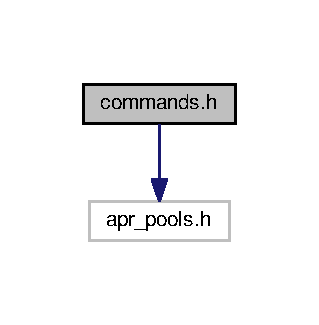
\includegraphics[width=153pt]{commands_8h__incl}
\end{center}
\end{figure}
This graph shows which files directly or indirectly include this file\+:\nopagebreak
\begin{figure}[H]
\begin{center}
\leavevmode
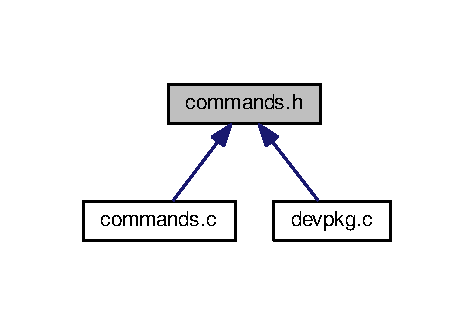
\includegraphics[width=228pt]{commands_8h__dep__incl}
\end{center}
\end{figure}
\subsection*{Macros}
\begin{DoxyCompactItemize}
\item 
\#define \hyperlink{commands_8h_ab9120c5dbc121bc45a0cdd133e291379}{D\+E\+P\+E\+N\+D\+S\+\_\+\+P\+A\+T\+H}~\char`\"{}/tmp/D\+E\+P\+E\+N\+D\+S\char`\"{}
\item 
\#define \hyperlink{commands_8h_a9c2aedcf20beed95d9f94e54a5b98c77}{T\+A\+R\+\_\+\+G\+Z\+\_\+\+S\+R\+C}~\char`\"{}/tmp/pkg-\/src.\+tar.\+gz\char`\"{}
\item 
\#define \hyperlink{commands_8h_af71a088f27cf2ef8f751d81273078c68}{T\+A\+R\+\_\+\+B\+Z2\+\_\+\+S\+R\+C}~\char`\"{}/tmp/pkg-\/src.\+tar.\+bz2\char`\"{}
\item 
\#define \hyperlink{commands_8h_a40ae373788da1701b1df883e62b46373}{B\+U\+I\+L\+D\+\_\+\+D\+I\+R}~\char`\"{}/tmp/pkg-\/build\char`\"{}
\item 
\#define \hyperlink{commands_8h_a8cabfe3e73eed8ee4083b7118086f140}{G\+I\+T\+\_\+\+P\+A\+T}~\char`\"{}$\ast$.git\char`\"{}
\item 
\#define \hyperlink{commands_8h_a358f5b64984880fa59ea893e449fc3bb}{D\+E\+P\+E\+N\+D\+\_\+\+P\+A\+T}~\char`\"{}$\ast$D\+E\+P\+E\+N\+D\+S\char`\"{}
\item 
\#define \hyperlink{commands_8h_afaa18bb2bbdb4a50196ec414bd0e1227}{T\+A\+R\+\_\+\+G\+Z\+\_\+\+P\+A\+T}~\char`\"{}$\ast$.tar.\+gz\char`\"{}
\item 
\#define \hyperlink{commands_8h_acc3e9a00f81bb887a0dfbf6648467e6b}{T\+A\+R\+\_\+\+B\+Z2\+\_\+\+P\+A\+T}~\char`\"{}$\ast$.tar.\+bz2\char`\"{}
\item 
\#define \hyperlink{commands_8h_ab780866c2a8435a305bc8fe7e6ee688a}{C\+O\+N\+F\+I\+G\+\_\+\+S\+C\+R\+I\+P\+T}~\char`\"{}/tmp/pkg-\/build/configure\char`\"{}
\end{DoxyCompactItemize}
\subsection*{Enumerations}
\begin{DoxyCompactItemize}
\item 
\hypertarget{commands_8h_a21e038f5b8958e203d28bc4f18472352}{}enum \hyperlink{commands_8h_a21e038f5b8958e203d28bc4f18472352}{Command\+Type} \{ \\*
{\bfseries C\+O\+M\+M\+A\+N\+D\+\_\+\+N\+O\+N\+E}, 
{\bfseries C\+O\+M\+M\+A\+N\+D\+\_\+\+I\+N\+S\+T\+A\+L\+L}, 
{\bfseries C\+O\+M\+M\+A\+N\+D\+\_\+\+L\+I\+S\+T}, 
{\bfseries C\+O\+M\+M\+A\+N\+D\+\_\+\+F\+E\+T\+C\+H}, 
\\*
{\bfseries C\+O\+M\+M\+A\+N\+D\+\_\+\+I\+N\+I\+T}, 
{\bfseries C\+O\+M\+M\+A\+M\+D\+\_\+\+B\+U\+I\+L\+D}, 
{\bfseries C\+O\+M\+M\+A\+M\+D\+\_\+\+D\+E\+P\+S}
 \}\label{commands_8h_a21e038f5b8958e203d28bc4f18472352}

\begin{DoxyCompactList}\small\item\em commands \end{DoxyCompactList}\end{DoxyCompactItemize}
\subsection*{Functions}
\begin{DoxyCompactItemize}
\item 
int \hyperlink{commands_8h_affbc6091a8bd093b418d1701bc2f7307}{Command\+\_\+fetch} (apr\+\_\+pool\+\_\+t $\ast$p, const char $\ast$url, int fetch\+\_\+only)
\begin{DoxyCompactList}\small\item\em fetch package from url \end{DoxyCompactList}\item 
int \hyperlink{commands_8h_af384b213993ba94ca4f7e0492a544135}{Command\+\_\+install} (apr\+\_\+pool\+\_\+t $\ast$p, const char $\ast$url, const char $\ast$configure\+\_\+opts, const char $\ast$make\+\_\+opts, const char $\ast$install\+\_\+opts)
\begin{DoxyCompactList}\small\item\em Install package command. \end{DoxyCompactList}\item 
int \hyperlink{commands_8h_a8f5695cbe4457871b9ac8a7f686e93e9}{Command\+\_\+depends} (apr\+\_\+pool\+\_\+t $\ast$p, const char $\ast$path)
\begin{DoxyCompactList}\small\item\em install all depends package for path \end{DoxyCompactList}\item 
int \hyperlink{commands_8h_a6910667dba531ef95fc0a445bdbf0141}{Command\+\_\+build} (apr\+\_\+pool\+\_\+t $\ast$p, const char $\ast$url, const char $\ast$configure\+\_\+opts, const char $\ast$make\+\_\+opts, const char $\ast$install\+\_\+opts)
\begin{DoxyCompactList}\small\item\em build package from url \end{DoxyCompactList}\end{DoxyCompactItemize}


\subsection{Detailed Description}
commands 

\begin{DoxyAuthor}{Author}
peter liu \href{mailto:peter.liu.work@gmail.com.tw}{\tt peter.\+liu.\+work@gmail.\+com.\+tw} 
\end{DoxyAuthor}
\begin{DoxyVersion}{Version}
0.\+0 
\end{DoxyVersion}
\begin{DoxyDate}{Date}
2016-\/04-\/13 
\end{DoxyDate}


\subsection{Macro Definition Documentation}
\hypertarget{commands_8h_a40ae373788da1701b1df883e62b46373}{}\index{commands.\+h@{commands.\+h}!B\+U\+I\+L\+D\+\_\+\+D\+I\+R@{B\+U\+I\+L\+D\+\_\+\+D\+I\+R}}
\index{B\+U\+I\+L\+D\+\_\+\+D\+I\+R@{B\+U\+I\+L\+D\+\_\+\+D\+I\+R}!commands.\+h@{commands.\+h}}
\subsubsection[{B\+U\+I\+L\+D\+\_\+\+D\+I\+R}]{\setlength{\rightskip}{0pt plus 5cm}\#define B\+U\+I\+L\+D\+\_\+\+D\+I\+R~\char`\"{}/tmp/pkg-\/build\char`\"{}}\label{commands_8h_a40ae373788da1701b1df883e62b46373}
package build directory \hypertarget{commands_8h_ab780866c2a8435a305bc8fe7e6ee688a}{}\index{commands.\+h@{commands.\+h}!C\+O\+N\+F\+I\+G\+\_\+\+S\+C\+R\+I\+P\+T@{C\+O\+N\+F\+I\+G\+\_\+\+S\+C\+R\+I\+P\+T}}
\index{C\+O\+N\+F\+I\+G\+\_\+\+S\+C\+R\+I\+P\+T@{C\+O\+N\+F\+I\+G\+\_\+\+S\+C\+R\+I\+P\+T}!commands.\+h@{commands.\+h}}
\subsubsection[{C\+O\+N\+F\+I\+G\+\_\+\+S\+C\+R\+I\+P\+T}]{\setlength{\rightskip}{0pt plus 5cm}\#define C\+O\+N\+F\+I\+G\+\_\+\+S\+C\+R\+I\+P\+T~\char`\"{}/tmp/pkg-\/build/configure\char`\"{}}\label{commands_8h_ab780866c2a8435a305bc8fe7e6ee688a}
package configure script file location \hypertarget{commands_8h_a358f5b64984880fa59ea893e449fc3bb}{}\index{commands.\+h@{commands.\+h}!D\+E\+P\+E\+N\+D\+\_\+\+P\+A\+T@{D\+E\+P\+E\+N\+D\+\_\+\+P\+A\+T}}
\index{D\+E\+P\+E\+N\+D\+\_\+\+P\+A\+T@{D\+E\+P\+E\+N\+D\+\_\+\+P\+A\+T}!commands.\+h@{commands.\+h}}
\subsubsection[{D\+E\+P\+E\+N\+D\+\_\+\+P\+A\+T}]{\setlength{\rightskip}{0pt plus 5cm}\#define D\+E\+P\+E\+N\+D\+\_\+\+P\+A\+T~\char`\"{}$\ast$D\+E\+P\+E\+N\+D\+S\char`\"{}}\label{commands_8h_a358f5b64984880fa59ea893e449fc3bb}
$\ast$.depends url pattern \hypertarget{commands_8h_ab9120c5dbc121bc45a0cdd133e291379}{}\index{commands.\+h@{commands.\+h}!D\+E\+P\+E\+N\+D\+S\+\_\+\+P\+A\+T\+H@{D\+E\+P\+E\+N\+D\+S\+\_\+\+P\+A\+T\+H}}
\index{D\+E\+P\+E\+N\+D\+S\+\_\+\+P\+A\+T\+H@{D\+E\+P\+E\+N\+D\+S\+\_\+\+P\+A\+T\+H}!commands.\+h@{commands.\+h}}
\subsubsection[{D\+E\+P\+E\+N\+D\+S\+\_\+\+P\+A\+T\+H}]{\setlength{\rightskip}{0pt plus 5cm}\#define D\+E\+P\+E\+N\+D\+S\+\_\+\+P\+A\+T\+H~\char`\"{}/tmp/D\+E\+P\+E\+N\+D\+S\char`\"{}}\label{commands_8h_ab9120c5dbc121bc45a0cdd133e291379}
depends directory \hypertarget{commands_8h_a8cabfe3e73eed8ee4083b7118086f140}{}\index{commands.\+h@{commands.\+h}!G\+I\+T\+\_\+\+P\+A\+T@{G\+I\+T\+\_\+\+P\+A\+T}}
\index{G\+I\+T\+\_\+\+P\+A\+T@{G\+I\+T\+\_\+\+P\+A\+T}!commands.\+h@{commands.\+h}}
\subsubsection[{G\+I\+T\+\_\+\+P\+A\+T}]{\setlength{\rightskip}{0pt plus 5cm}\#define G\+I\+T\+\_\+\+P\+A\+T~\char`\"{}$\ast$.git\char`\"{}}\label{commands_8h_a8cabfe3e73eed8ee4083b7118086f140}
$\ast$.git url pattern \hypertarget{commands_8h_acc3e9a00f81bb887a0dfbf6648467e6b}{}\index{commands.\+h@{commands.\+h}!T\+A\+R\+\_\+\+B\+Z2\+\_\+\+P\+A\+T@{T\+A\+R\+\_\+\+B\+Z2\+\_\+\+P\+A\+T}}
\index{T\+A\+R\+\_\+\+B\+Z2\+\_\+\+P\+A\+T@{T\+A\+R\+\_\+\+B\+Z2\+\_\+\+P\+A\+T}!commands.\+h@{commands.\+h}}
\subsubsection[{T\+A\+R\+\_\+\+B\+Z2\+\_\+\+P\+A\+T}]{\setlength{\rightskip}{0pt plus 5cm}\#define T\+A\+R\+\_\+\+B\+Z2\+\_\+\+P\+A\+T~\char`\"{}$\ast$.tar.\+bz2\char`\"{}}\label{commands_8h_acc3e9a00f81bb887a0dfbf6648467e6b}
$\ast$.tar.\+bz2 url pattern \hypertarget{commands_8h_af71a088f27cf2ef8f751d81273078c68}{}\index{commands.\+h@{commands.\+h}!T\+A\+R\+\_\+\+B\+Z2\+\_\+\+S\+R\+C@{T\+A\+R\+\_\+\+B\+Z2\+\_\+\+S\+R\+C}}
\index{T\+A\+R\+\_\+\+B\+Z2\+\_\+\+S\+R\+C@{T\+A\+R\+\_\+\+B\+Z2\+\_\+\+S\+R\+C}!commands.\+h@{commands.\+h}}
\subsubsection[{T\+A\+R\+\_\+\+B\+Z2\+\_\+\+S\+R\+C}]{\setlength{\rightskip}{0pt plus 5cm}\#define T\+A\+R\+\_\+\+B\+Z2\+\_\+\+S\+R\+C~\char`\"{}/tmp/pkg-\/src.\+tar.\+bz2\char`\"{}}\label{commands_8h_af71a088f27cf2ef8f751d81273078c68}
$\ast$.tar.\+bz2 package source directory \hypertarget{commands_8h_afaa18bb2bbdb4a50196ec414bd0e1227}{}\index{commands.\+h@{commands.\+h}!T\+A\+R\+\_\+\+G\+Z\+\_\+\+P\+A\+T@{T\+A\+R\+\_\+\+G\+Z\+\_\+\+P\+A\+T}}
\index{T\+A\+R\+\_\+\+G\+Z\+\_\+\+P\+A\+T@{T\+A\+R\+\_\+\+G\+Z\+\_\+\+P\+A\+T}!commands.\+h@{commands.\+h}}
\subsubsection[{T\+A\+R\+\_\+\+G\+Z\+\_\+\+P\+A\+T}]{\setlength{\rightskip}{0pt plus 5cm}\#define T\+A\+R\+\_\+\+G\+Z\+\_\+\+P\+A\+T~\char`\"{}$\ast$.tar.\+gz\char`\"{}}\label{commands_8h_afaa18bb2bbdb4a50196ec414bd0e1227}
$\ast$.tar.\+gz url pattern \hypertarget{commands_8h_a9c2aedcf20beed95d9f94e54a5b98c77}{}\index{commands.\+h@{commands.\+h}!T\+A\+R\+\_\+\+G\+Z\+\_\+\+S\+R\+C@{T\+A\+R\+\_\+\+G\+Z\+\_\+\+S\+R\+C}}
\index{T\+A\+R\+\_\+\+G\+Z\+\_\+\+S\+R\+C@{T\+A\+R\+\_\+\+G\+Z\+\_\+\+S\+R\+C}!commands.\+h@{commands.\+h}}
\subsubsection[{T\+A\+R\+\_\+\+G\+Z\+\_\+\+S\+R\+C}]{\setlength{\rightskip}{0pt plus 5cm}\#define T\+A\+R\+\_\+\+G\+Z\+\_\+\+S\+R\+C~\char`\"{}/tmp/pkg-\/src.\+tar.\+gz\char`\"{}}\label{commands_8h_a9c2aedcf20beed95d9f94e54a5b98c77}
$\ast$.tar.\+gz package source directory 

\subsection{Function Documentation}
\hypertarget{commands_8h_a6910667dba531ef95fc0a445bdbf0141}{}\index{commands.\+h@{commands.\+h}!Command\+\_\+build@{Command\+\_\+build}}
\index{Command\+\_\+build@{Command\+\_\+build}!commands.\+h@{commands.\+h}}
\subsubsection[{Command\+\_\+build}]{\setlength{\rightskip}{0pt plus 5cm}int Command\+\_\+build (
\begin{DoxyParamCaption}
\item[{apr\+\_\+pool\+\_\+t $\ast$}]{p, }
\item[{const char $\ast$}]{url, }
\item[{const char $\ast$}]{configure\+\_\+opts, }
\item[{const char $\ast$}]{make\+\_\+opts, }
\item[{const char $\ast$}]{install\+\_\+opts}
\end{DoxyParamCaption}
)}\label{commands_8h_a6910667dba531ef95fc0a445bdbf0141}


build package from url 


\begin{DoxyParams}{Parameters}
{\em p} & A\+P\+R pool \\
\hline
{\em url} & url to build \\
\hline
{\em configure\+\_\+opts} & configure options \\
\hline
{\em make\+\_\+opts} & make options \\
\hline
{\em install\+\_\+opts} & install options\\
\hline
\end{DoxyParams}
\begin{DoxyReturn}{Returns}
{\bfseries 0}\+: build, make, install, cleanup, and database update successfully ~\newline
{\bfseries -\/1}\+: otherwise 
\end{DoxyReturn}
\hypertarget{commands_8h_a8f5695cbe4457871b9ac8a7f686e93e9}{}\index{commands.\+h@{commands.\+h}!Command\+\_\+depends@{Command\+\_\+depends}}
\index{Command\+\_\+depends@{Command\+\_\+depends}!commands.\+h@{commands.\+h}}
\subsubsection[{Command\+\_\+depends}]{\setlength{\rightskip}{0pt plus 5cm}int Command\+\_\+depends (
\begin{DoxyParamCaption}
\item[{apr\+\_\+pool\+\_\+t $\ast$}]{p, }
\item[{const char $\ast$}]{path}
\end{DoxyParamCaption}
)}\label{commands_8h_a8f5695cbe4457871b9ac8a7f686e93e9}


install all depends package for path 


\begin{DoxyParams}{Parameters}
{\em p} & A\+P\+R pool \\
\hline
{\em path} & depends file path which contains a url per line\\
\hline
\end{DoxyParams}
\begin{DoxyReturn}{Returns}
{\bfseries 0}\+: All dependes are installed successfully ~\newline
{\bfseries -\/1}\+: Otherwise 
\end{DoxyReturn}
\hypertarget{commands_8h_affbc6091a8bd093b418d1701bc2f7307}{}\index{commands.\+h@{commands.\+h}!Command\+\_\+fetch@{Command\+\_\+fetch}}
\index{Command\+\_\+fetch@{Command\+\_\+fetch}!commands.\+h@{commands.\+h}}
\subsubsection[{Command\+\_\+fetch}]{\setlength{\rightskip}{0pt plus 5cm}int Command\+\_\+fetch (
\begin{DoxyParamCaption}
\item[{apr\+\_\+pool\+\_\+t $\ast$}]{p, }
\item[{const char $\ast$}]{url, }
\item[{int}]{fetch\+\_\+only}
\end{DoxyParamCaption}
)}\label{commands_8h_affbc6091a8bd093b418d1701bc2f7307}


fetch package from url 


\begin{DoxyParams}{Parameters}
{\em p} & A\+P\+R pool \\
\hline
{\em url} & url to fetch \\
\hline
{\em fetch\+\_\+only} & fetch only\\
\hline
\end{DoxyParams}
\begin{DoxyReturn}{Returns}
{\bfseries 1}\+: fetch success, need to build \& install ~\newline
{\bfseries 0}\+: fetch success, nothing to do ~\newline
{\bfseries -\/1}\+: fetch error 
\end{DoxyReturn}
\hypertarget{commands_8h_af384b213993ba94ca4f7e0492a544135}{}\index{commands.\+h@{commands.\+h}!Command\+\_\+install@{Command\+\_\+install}}
\index{Command\+\_\+install@{Command\+\_\+install}!commands.\+h@{commands.\+h}}
\subsubsection[{Command\+\_\+install}]{\setlength{\rightskip}{0pt plus 5cm}int Command\+\_\+install (
\begin{DoxyParamCaption}
\item[{apr\+\_\+pool\+\_\+t $\ast$}]{p, }
\item[{const char $\ast$}]{url, }
\item[{const char $\ast$}]{configure\+\_\+opts, }
\item[{const char $\ast$}]{make\+\_\+opts, }
\item[{const char $\ast$}]{install\+\_\+opts}
\end{DoxyParamCaption}
)}\label{commands_8h_af384b213993ba94ca4f7e0492a544135}


Install package command. 

The package come from input parameter \+: url


\begin{DoxyParams}{Parameters}
{\em p} & A\+P\+R pool \\
\hline
{\em url} & package url \\
\hline
{\em configure\+\_\+opts} & configure options \\
\hline
{\em make\+\_\+opts} & make options \\
\hline
{\em install\+\_\+opts} & install options\\
\hline
\end{DoxyParams}
\begin{DoxyReturn}{Returns}
{\bfseries 0}\+: install sucess ~\newline
{\bfseries -\/1}\+: install fail 
\end{DoxyReturn}

\hypertarget{db_8c}{}\section{db.\+c File Reference}
\label{db_8c}\index{db.\+c@{db.\+c}}


simple data base  


{\ttfamily \#include $<$unistd.\+h$>$}\\*
{\ttfamily \#include $<$apr\+\_\+errno.\+h$>$}\\*
{\ttfamily \#include $<$apr\+\_\+file\+\_\+io.\+h$>$}\\*
{\ttfamily \#include \char`\"{}db.\+h\char`\"{}}\\*
{\ttfamily \#include \char`\"{}bstrlib.\+h\char`\"{}}\\*
{\ttfamily \#include \char`\"{}../../common/include/dbg.\+h\char`\"{}}\\*
Include dependency graph for db.\+c\+:\nopagebreak
\begin{figure}[H]
\begin{center}
\leavevmode
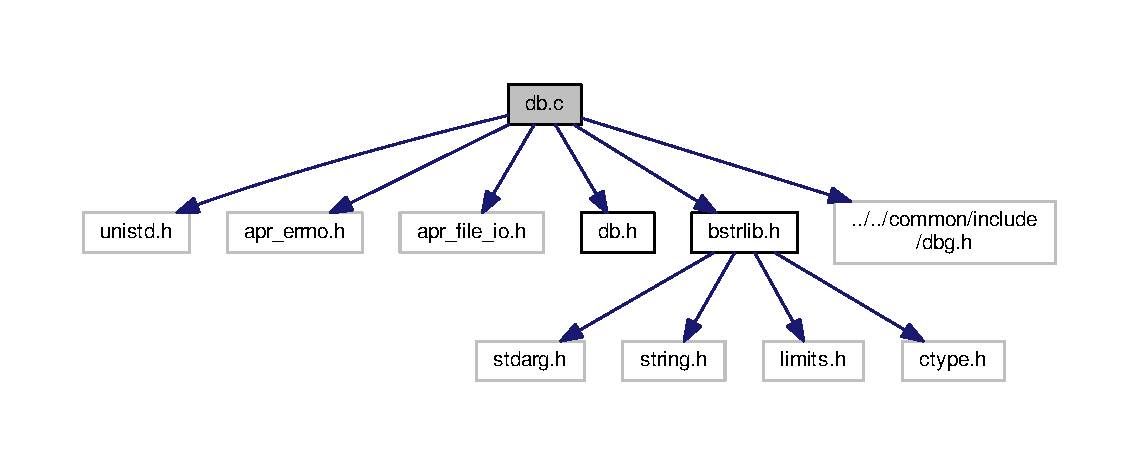
\includegraphics[width=350pt]{db_8c__incl}
\end{center}
\end{figure}
\subsection*{Functions}
\begin{DoxyCompactItemize}
\item 
int \hyperlink{db_8c_aa82653649df4b8d4f53bb91547e3cd86}{D\+B\+\_\+update} (const char $\ast$url)
\begin{DoxyCompactList}\small\item\em database update \end{DoxyCompactList}\item 
int \hyperlink{db_8c_a191bcd1e638af8c3f86e7aafd8483315}{D\+B\+\_\+find} (const char $\ast$url)
\begin{DoxyCompactList}\small\item\em find database to input url \end{DoxyCompactList}\item 
int \hyperlink{db_8c_a68f3866a342eb53891f951753294b36a}{D\+B\+\_\+init} (void)
\begin{DoxyCompactList}\small\item\em database initialize \end{DoxyCompactList}\item 
int \hyperlink{db_8c_a664f1e650653baa531fbd0de70ad6c5e}{D\+B\+\_\+list} (void)
\begin{DoxyCompactList}\small\item\em database list it\textquotesingle{}s contents \end{DoxyCompactList}\end{DoxyCompactItemize}


\subsection{Detailed Description}
simple data base 

\begin{DoxyAuthor}{Author}
peter liu \href{mailto:peter.liu.work@gmail.com.tw}{\tt peter.\+liu.\+work@gmail.\+com.\+tw} 
\end{DoxyAuthor}
\begin{DoxyVersion}{Version}
0.\+0 
\end{DoxyVersion}
\begin{DoxyDate}{Date}
2016-\/04-\/10 
\end{DoxyDate}


\subsection{Function Documentation}
\hypertarget{db_8c_a191bcd1e638af8c3f86e7aafd8483315}{}\index{db.\+c@{db.\+c}!D\+B\+\_\+find@{D\+B\+\_\+find}}
\index{D\+B\+\_\+find@{D\+B\+\_\+find}!db.\+c@{db.\+c}}
\subsubsection[{D\+B\+\_\+find}]{\setlength{\rightskip}{0pt plus 5cm}int D\+B\+\_\+find (
\begin{DoxyParamCaption}
\item[{const char $\ast$}]{url}
\end{DoxyParamCaption}
)}\label{db_8c_a191bcd1e638af8c3f86e7aafd8483315}


find database to input url 


\begin{DoxyParams}{Parameters}
{\em url} & usl to find\\
\hline
\end{DoxyParams}
\begin{DoxyReturn}{Returns}
{\bfseries 0}\+: url can\textquotesingle{}t find in database ~\newline
{\bfseries 1}\+: url find in data base ~\newline
{\bfseries -\/1}\+: error -\/ url is N\+U\+L\+L ~\newline
{\bfseries -\/2}\+: bstring allocate memory failed ~\newline
{\bfseries -\/3}\+: error -\/ datebase can\textquotesingle{}t load 
\end{DoxyReturn}
\hypertarget{db_8c_a68f3866a342eb53891f951753294b36a}{}\index{db.\+c@{db.\+c}!D\+B\+\_\+init@{D\+B\+\_\+init}}
\index{D\+B\+\_\+init@{D\+B\+\_\+init}!db.\+c@{db.\+c}}
\subsubsection[{D\+B\+\_\+init}]{\setlength{\rightskip}{0pt plus 5cm}int D\+B\+\_\+init (
\begin{DoxyParamCaption}
\item[{void}]{}
\end{DoxyParamCaption}
)}\label{db_8c_a68f3866a342eb53891f951753294b36a}


database initialize 

\begin{DoxyReturn}{Returns}
{\bfseries 0}\+: database initialize successfully ~\newline
{\bfseries -\/1}\+: Otherwies 
\end{DoxyReturn}
\hypertarget{db_8c_a664f1e650653baa531fbd0de70ad6c5e}{}\index{db.\+c@{db.\+c}!D\+B\+\_\+list@{D\+B\+\_\+list}}
\index{D\+B\+\_\+list@{D\+B\+\_\+list}!db.\+c@{db.\+c}}
\subsubsection[{D\+B\+\_\+list}]{\setlength{\rightskip}{0pt plus 5cm}int D\+B\+\_\+list (
\begin{DoxyParamCaption}
\item[{void}]{}
\end{DoxyParamCaption}
)}\label{db_8c_a664f1e650653baa531fbd0de70ad6c5e}


database list it\textquotesingle{}s contents 

\begin{DoxyReturn}{Returns}
{\bfseries 0}\+: List success ~\newline
{\bfseries -\/1}\+: Otherwise 
\end{DoxyReturn}
\hypertarget{db_8c_aa82653649df4b8d4f53bb91547e3cd86}{}\index{db.\+c@{db.\+c}!D\+B\+\_\+update@{D\+B\+\_\+update}}
\index{D\+B\+\_\+update@{D\+B\+\_\+update}!db.\+c@{db.\+c}}
\subsubsection[{D\+B\+\_\+update}]{\setlength{\rightskip}{0pt plus 5cm}int D\+B\+\_\+update (
\begin{DoxyParamCaption}
\item[{const char $\ast$}]{url}
\end{DoxyParamCaption}
)}\label{db_8c_aa82653649df4b8d4f53bb91547e3cd86}


database update 


\begin{DoxyParams}{Parameters}
{\em url} & url to update\\
\hline
\end{DoxyParams}
\begin{DoxyReturn}{Returns}
{\bfseries 0}\+: database update success ~\newline
{\bfseries -\/1}\+: database update fail 
\end{DoxyReturn}

\hypertarget{db_8h}{}\section{db.\+h File Reference}
\label{db_8h}\index{db.\+h@{db.\+h}}


database  


This graph shows which files directly or indirectly include this file\+:\nopagebreak
\begin{figure}[H]
\begin{center}
\leavevmode
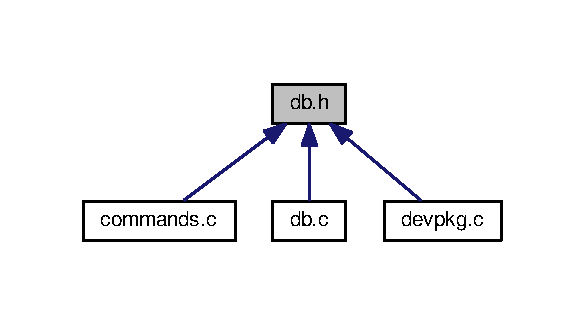
\includegraphics[width=281pt]{db_8h__dep__incl}
\end{center}
\end{figure}
\subsection*{Macros}
\begin{DoxyCompactItemize}
\item 
\#define \hyperlink{db_8h_aee925031172607ff8d5cf8b68374bd7f}{D\+B\+\_\+\+F\+I\+L\+E}~\char`\"{}/usr/local/.devpkg/db\char`\"{}
\item 
\#define \hyperlink{db_8h_ae23024310783ea0e70a78c70b8896a2e}{D\+B\+\_\+\+D\+I\+R}~\char`\"{}/usr/local/.devpkg\char`\"{}
\end{DoxyCompactItemize}
\subsection*{Functions}
\begin{DoxyCompactItemize}
\item 
int \hyperlink{db_8h_a68f3866a342eb53891f951753294b36a}{D\+B\+\_\+init} (void)
\begin{DoxyCompactList}\small\item\em database initialize \end{DoxyCompactList}\item 
int \hyperlink{db_8h_a664f1e650653baa531fbd0de70ad6c5e}{D\+B\+\_\+list} (void)
\begin{DoxyCompactList}\small\item\em database list it\textquotesingle{}s contents \end{DoxyCompactList}\item 
int \hyperlink{db_8h_aa82653649df4b8d4f53bb91547e3cd86}{D\+B\+\_\+update} (const char $\ast$url)
\begin{DoxyCompactList}\small\item\em database update \end{DoxyCompactList}\item 
int \hyperlink{db_8h_a191bcd1e638af8c3f86e7aafd8483315}{D\+B\+\_\+find} (const char $\ast$url)
\begin{DoxyCompactList}\small\item\em find database to input url \end{DoxyCompactList}\end{DoxyCompactItemize}


\subsection{Detailed Description}
database 

\begin{DoxyAuthor}{Author}
peter liu \href{mailto:peter.liu.work@gmail.com.tw}{\tt peter.\+liu.\+work@gmail.\+com.\+tw} 
\end{DoxyAuthor}
\begin{DoxyVersion}{Version}
0.\+0 
\end{DoxyVersion}
\begin{DoxyDate}{Date}
2016-\/04-\/13 
\end{DoxyDate}


\subsection{Macro Definition Documentation}
\hypertarget{db_8h_ae23024310783ea0e70a78c70b8896a2e}{}\index{db.\+h@{db.\+h}!D\+B\+\_\+\+D\+I\+R@{D\+B\+\_\+\+D\+I\+R}}
\index{D\+B\+\_\+\+D\+I\+R@{D\+B\+\_\+\+D\+I\+R}!db.\+h@{db.\+h}}
\subsubsection[{D\+B\+\_\+\+D\+I\+R}]{\setlength{\rightskip}{0pt plus 5cm}\#define D\+B\+\_\+\+D\+I\+R~\char`\"{}/usr/local/.devpkg\char`\"{}}\label{db_8h_ae23024310783ea0e70a78c70b8896a2e}
database directory path \hypertarget{db_8h_aee925031172607ff8d5cf8b68374bd7f}{}\index{db.\+h@{db.\+h}!D\+B\+\_\+\+F\+I\+L\+E@{D\+B\+\_\+\+F\+I\+L\+E}}
\index{D\+B\+\_\+\+F\+I\+L\+E@{D\+B\+\_\+\+F\+I\+L\+E}!db.\+h@{db.\+h}}
\subsubsection[{D\+B\+\_\+\+F\+I\+L\+E}]{\setlength{\rightskip}{0pt plus 5cm}\#define D\+B\+\_\+\+F\+I\+L\+E~\char`\"{}/usr/local/.devpkg/db\char`\"{}}\label{db_8h_aee925031172607ff8d5cf8b68374bd7f}
databae file path 

\subsection{Function Documentation}
\hypertarget{db_8h_a191bcd1e638af8c3f86e7aafd8483315}{}\index{db.\+h@{db.\+h}!D\+B\+\_\+find@{D\+B\+\_\+find}}
\index{D\+B\+\_\+find@{D\+B\+\_\+find}!db.\+h@{db.\+h}}
\subsubsection[{D\+B\+\_\+find}]{\setlength{\rightskip}{0pt plus 5cm}int D\+B\+\_\+find (
\begin{DoxyParamCaption}
\item[{const char $\ast$}]{url}
\end{DoxyParamCaption}
)}\label{db_8h_a191bcd1e638af8c3f86e7aafd8483315}


find database to input url 


\begin{DoxyParams}{Parameters}
{\em url} & usl to find\\
\hline
\end{DoxyParams}
\begin{DoxyReturn}{Returns}
{\bfseries 0}\+: url can\textquotesingle{}t find in database ~\newline
{\bfseries 1}\+: url find in data base ~\newline
{\bfseries -\/1}\+: error -\/ url is N\+U\+L\+L ~\newline
{\bfseries -\/2}\+: bstring allocate memory failed ~\newline
{\bfseries -\/3}\+: error -\/ datebase can\textquotesingle{}t load 
\end{DoxyReturn}
\hypertarget{db_8h_a68f3866a342eb53891f951753294b36a}{}\index{db.\+h@{db.\+h}!D\+B\+\_\+init@{D\+B\+\_\+init}}
\index{D\+B\+\_\+init@{D\+B\+\_\+init}!db.\+h@{db.\+h}}
\subsubsection[{D\+B\+\_\+init}]{\setlength{\rightskip}{0pt plus 5cm}int D\+B\+\_\+init (
\begin{DoxyParamCaption}
\item[{void}]{}
\end{DoxyParamCaption}
)}\label{db_8h_a68f3866a342eb53891f951753294b36a}


database initialize 

\begin{DoxyReturn}{Returns}
{\bfseries 0}\+: database initialize successfully ~\newline
{\bfseries -\/1}\+: Otherwies 
\end{DoxyReturn}
\hypertarget{db_8h_a664f1e650653baa531fbd0de70ad6c5e}{}\index{db.\+h@{db.\+h}!D\+B\+\_\+list@{D\+B\+\_\+list}}
\index{D\+B\+\_\+list@{D\+B\+\_\+list}!db.\+h@{db.\+h}}
\subsubsection[{D\+B\+\_\+list}]{\setlength{\rightskip}{0pt plus 5cm}int D\+B\+\_\+list (
\begin{DoxyParamCaption}
\item[{void}]{}
\end{DoxyParamCaption}
)}\label{db_8h_a664f1e650653baa531fbd0de70ad6c5e}


database list it\textquotesingle{}s contents 

\begin{DoxyReturn}{Returns}
{\bfseries 0}\+: List success ~\newline
{\bfseries -\/1}\+: Otherwise 
\end{DoxyReturn}
\hypertarget{db_8h_aa82653649df4b8d4f53bb91547e3cd86}{}\index{db.\+h@{db.\+h}!D\+B\+\_\+update@{D\+B\+\_\+update}}
\index{D\+B\+\_\+update@{D\+B\+\_\+update}!db.\+h@{db.\+h}}
\subsubsection[{D\+B\+\_\+update}]{\setlength{\rightskip}{0pt plus 5cm}int D\+B\+\_\+update (
\begin{DoxyParamCaption}
\item[{const char $\ast$}]{url}
\end{DoxyParamCaption}
)}\label{db_8h_aa82653649df4b8d4f53bb91547e3cd86}


database update 


\begin{DoxyParams}{Parameters}
{\em url} & url to update\\
\hline
\end{DoxyParams}
\begin{DoxyReturn}{Returns}
{\bfseries 0}\+: database update success ~\newline
{\bfseries -\/1}\+: database update fail 
\end{DoxyReturn}

\hypertarget{devpkg_8c}{}\section{devpkg.\+c File Reference}
\label{devpkg_8c}\index{devpkg.\+c@{devpkg.\+c}}


Packages manage main function.  


{\ttfamily \#include $<$stdio.\+h$>$}\\*
{\ttfamily \#include $<$stdlib.\+h$>$}\\*
{\ttfamily \#include $<$string.\+h$>$}\\*
{\ttfamily \#include $<$apr\+\_\+general.\+h$>$}\\*
{\ttfamily \#include $<$apr\+\_\+getopt.\+h$>$}\\*
{\ttfamily \#include $<$apr\+\_\+strings.\+h$>$}\\*
{\ttfamily \#include $<$apr\+\_\+lib.\+h$>$}\\*
{\ttfamily \#include \char`\"{}../../common/include/dbg.\+h\char`\"{}}\\*
{\ttfamily \#include \char`\"{}db.\+h\char`\"{}}\\*
{\ttfamily \#include \char`\"{}commands.\+h\char`\"{}}\\*
Include dependency graph for devpkg.\+c\+:\nopagebreak
\begin{figure}[H]
\begin{center}
\leavevmode
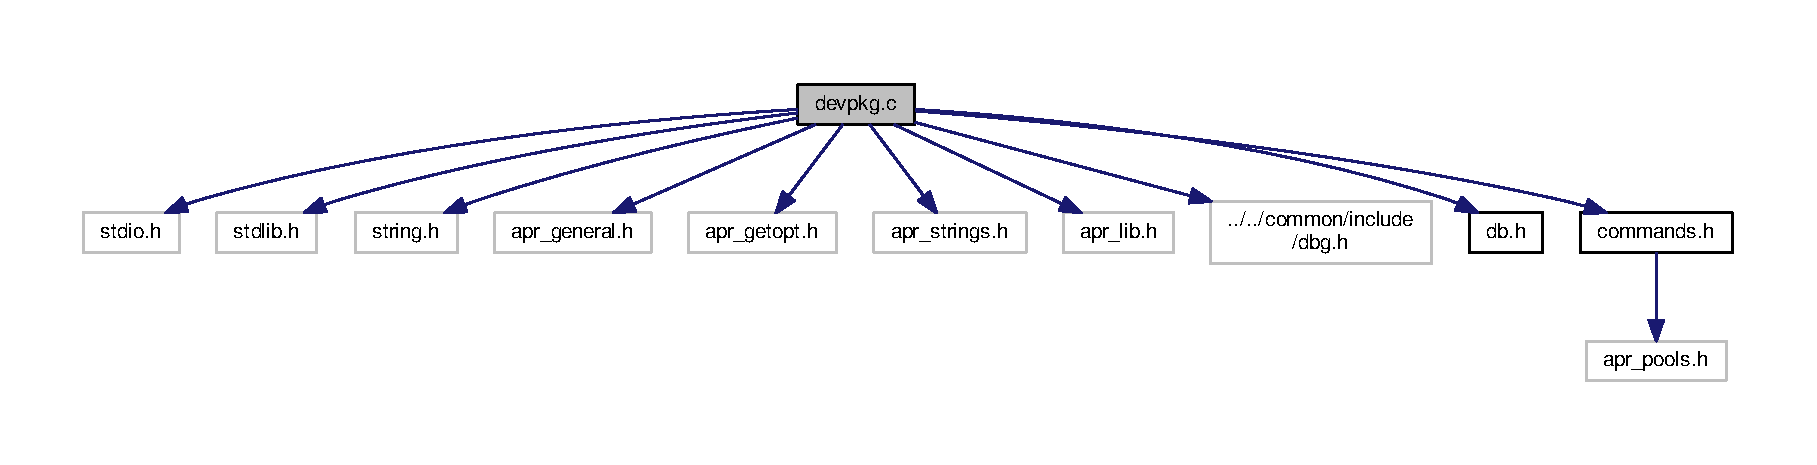
\includegraphics[width=350pt]{devpkg_8c__incl}
\end{center}
\end{figure}
\subsection*{Macros}
\begin{DoxyCompactItemize}
\item 
\#define \hyperlink{devpkg_8c_af7ef5f2536930730d1baa596db61c0f9}{C\+L\+I\+\_\+\+C\+M\+D\+\_\+\+E\+R\+R\+O\+R\+\_\+\+U\+S\+A\+G\+E\+\_\+\+S\+T\+R\+I\+N\+G}~\char`\"{}Invail command given.\textbackslash{}n\textbackslash{}t\+Usage\+: \%s -\/I url $\vert$ -\/L $\vert$ -\/c url $\vert$ -\/m url $\vert$ -\/i url $\vert$ -\/S $\vert$ -\/ F url $\vert$ -\/B url\char`\"{}, argv\mbox{[}0\mbox{]}
\end{DoxyCompactItemize}
\subsection*{Functions}
\begin{DoxyCompactItemize}
\item 
int \hyperlink{devpkg_8c_ac3e5abe2b43f4085d248ea8728fd45b9}{main} (int argc, const char const $\ast$argv\mbox{[}$\,$\mbox{]})
\begin{DoxyCompactList}\small\item\em main function \end{DoxyCompactList}\end{DoxyCompactItemize}
\subsection*{Variables}
\begin{DoxyCompactItemize}
\item 
const char const $\ast$ \hyperlink{devpkg_8c_a4ad9a452e6dcd0b44079e4e68716663a}{Command\+\_\+type\+\_\+names} \mbox{[}$\,$\mbox{]}
\begin{DoxyCompactList}\small\item\em command name string for debug only \end{DoxyCompactList}\end{DoxyCompactItemize}


\subsection{Detailed Description}
Packages manage main function. 

\begin{DoxyAuthor}{Author}
peter liu \href{mailto:peter.liu.work@gmail.com.tw}{\tt peter.\+liu.\+work@gmail.\+com.\+tw} 
\end{DoxyAuthor}
\begin{DoxyVersion}{Version}
0.\+0 
\end{DoxyVersion}
\begin{DoxyDate}{Date}
2016-\/04-\/13 
\end{DoxyDate}


\subsection{Macro Definition Documentation}
\hypertarget{devpkg_8c_af7ef5f2536930730d1baa596db61c0f9}{}\index{devpkg.\+c@{devpkg.\+c}!C\+L\+I\+\_\+\+C\+M\+D\+\_\+\+E\+R\+R\+O\+R\+\_\+\+U\+S\+A\+G\+E\+\_\+\+S\+T\+R\+I\+N\+G@{C\+L\+I\+\_\+\+C\+M\+D\+\_\+\+E\+R\+R\+O\+R\+\_\+\+U\+S\+A\+G\+E\+\_\+\+S\+T\+R\+I\+N\+G}}
\index{C\+L\+I\+\_\+\+C\+M\+D\+\_\+\+E\+R\+R\+O\+R\+\_\+\+U\+S\+A\+G\+E\+\_\+\+S\+T\+R\+I\+N\+G@{C\+L\+I\+\_\+\+C\+M\+D\+\_\+\+E\+R\+R\+O\+R\+\_\+\+U\+S\+A\+G\+E\+\_\+\+S\+T\+R\+I\+N\+G}!devpkg.\+c@{devpkg.\+c}}
\subsubsection[{C\+L\+I\+\_\+\+C\+M\+D\+\_\+\+E\+R\+R\+O\+R\+\_\+\+U\+S\+A\+G\+E\+\_\+\+S\+T\+R\+I\+N\+G}]{\setlength{\rightskip}{0pt plus 5cm}\#define C\+L\+I\+\_\+\+C\+M\+D\+\_\+\+E\+R\+R\+O\+R\+\_\+\+U\+S\+A\+G\+E\+\_\+\+S\+T\+R\+I\+N\+G~\char`\"{}Invail command given.\textbackslash{}n\textbackslash{}t\+Usage\+: \%s -\/I url $\vert$ -\/L $\vert$ -\/c url $\vert$ -\/m url $\vert$ -\/i url $\vert$ -\/S $\vert$ -\/ F url $\vert$ -\/B url\char`\"{}, argv\mbox{[}0\mbox{]}}\label{devpkg_8c_af7ef5f2536930730d1baa596db61c0f9}
command line error message\+: devpkg usage 

\subsection{Function Documentation}
\hypertarget{devpkg_8c_ac3e5abe2b43f4085d248ea8728fd45b9}{}\index{devpkg.\+c@{devpkg.\+c}!main@{main}}
\index{main@{main}!devpkg.\+c@{devpkg.\+c}}
\subsubsection[{main}]{\setlength{\rightskip}{0pt plus 5cm}int main (
\begin{DoxyParamCaption}
\item[{int}]{argc, }
\item[{const char const $\ast$}]{argv\mbox{[}$\,$\mbox{]}}
\end{DoxyParamCaption}
)}\label{devpkg_8c_ac3e5abe2b43f4085d248ea8728fd45b9}


main function 


\begin{DoxyParams}{Parameters}
{\em argc} & \\
\hline
{\em argv\mbox{[}$\,$\mbox{]}} & \\
\hline
\end{DoxyParams}
\begin{DoxyReturn}{Returns}

\end{DoxyReturn}


\subsection{Variable Documentation}
\hypertarget{devpkg_8c_a4ad9a452e6dcd0b44079e4e68716663a}{}\index{devpkg.\+c@{devpkg.\+c}!Command\+\_\+type\+\_\+names@{Command\+\_\+type\+\_\+names}}
\index{Command\+\_\+type\+\_\+names@{Command\+\_\+type\+\_\+names}!devpkg.\+c@{devpkg.\+c}}
\subsubsection[{Command\+\_\+type\+\_\+names}]{\setlength{\rightskip}{0pt plus 5cm}const char const$\ast$ Command\+\_\+type\+\_\+names\mbox{[}$\,$\mbox{]}}\label{devpkg_8c_a4ad9a452e6dcd0b44079e4e68716663a}
{\bfseries Initial value\+:}
\begin{DoxyCode}
= \{
    \textcolor{stringliteral}{"COMMAND\_NONE"},
    \textcolor{stringliteral}{"COMMAND\_INSTALL"},
    \textcolor{stringliteral}{"COMMAND\_LIST"},
    \textcolor{stringliteral}{"COMMAND\_FETCH"},
    \textcolor{stringliteral}{"COMMAND\_INIT"},
    \textcolor{stringliteral}{"COMMAMD\_BUILD"},
    \textcolor{stringliteral}{"COMMAMD\_DEPS"}
\}
\end{DoxyCode}


command name string for debug only 


\hypertarget{shell_8c}{}\section{shell.\+c File Reference}
\label{shell_8c}\index{shell.\+c@{shell.\+c}}


shell  


{\ttfamily \#include \char`\"{}shell.\+h\char`\"{}}\\*
{\ttfamily \#include \char`\"{}../../common/include/dbg.\+h\char`\"{}}\\*
{\ttfamily \#include $<$stdarg.\+h$>$}\\*
Include dependency graph for shell.\+c\+:\nopagebreak
\begin{figure}[H]
\begin{center}
\leavevmode
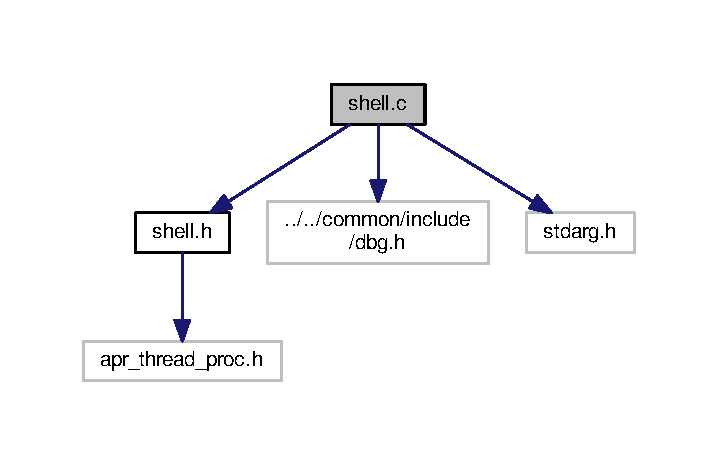
\includegraphics[width=345pt]{shell_8c__incl}
\end{center}
\end{figure}
\subsection*{Functions}
\begin{DoxyCompactItemize}
\item 
int \hyperlink{shell_8c_aff9ad8e697131563bcb0071b242a338d}{Shell\+\_\+exec} (\hyperlink{structShell}{Shell} template,...)
\begin{DoxyCompactList}\small\item\em shell execute \end{DoxyCompactList}\item 
int \hyperlink{shell_8c_acda27d63b5d5da99f9b12d52f376b006}{Shell\+\_\+run} (apr\+\_\+pool\+\_\+t $\ast$p, \hyperlink{structShell}{Shell} $\ast$cmd)
\begin{DoxyCompactList}\small\item\em shell run \end{DoxyCompactList}\end{DoxyCompactItemize}
\subsection*{Variables}
\begin{DoxyCompactItemize}
\item 
\hyperlink{structShell}{Shell} {\bfseries C\+L\+E\+A\+N\+U\+P\+\_\+\+S\+H}
\item 
\hyperlink{structShell}{Shell} {\bfseries G\+I\+T\+\_\+\+S\+H}
\item 
\hyperlink{structShell}{Shell} {\bfseries T\+A\+R\+\_\+\+B\+Z2\+\_\+\+S\+H}
\item 
\hyperlink{structShell}{Shell} {\bfseries T\+A\+R\+\_\+\+G\+Z\+\_\+\+S\+H}
\item 
\hyperlink{structShell}{Shell} {\bfseries C\+U\+R\+L\+\_\+\+S\+H}
\item 
\hyperlink{structShell}{Shell} {\bfseries C\+O\+N\+F\+I\+G\+U\+R\+E\+\_\+\+S\+H}
\item 
\hyperlink{structShell}{Shell} {\bfseries M\+A\+K\+E\+\_\+\+S\+H}
\item 
\hyperlink{structShell}{Shell} {\bfseries I\+N\+S\+T\+A\+L\+L\+\_\+\+S\+H}
\end{DoxyCompactItemize}


\subsection{Detailed Description}
shell 

\begin{DoxyAuthor}{Author}
peter liu \href{mailto:peter.liu.work@gmail.com.tw}{\tt peter.\+liu.\+work@gmail.\+com.\+tw} 
\end{DoxyAuthor}
\begin{DoxyVersion}{Version}
0.\+0 
\end{DoxyVersion}
\begin{DoxyDate}{Date}
2016-\/04-\/10 
\end{DoxyDate}


\subsection{Function Documentation}
\hypertarget{shell_8c_aff9ad8e697131563bcb0071b242a338d}{}\index{shell.\+c@{shell.\+c}!Shell\+\_\+exec@{Shell\+\_\+exec}}
\index{Shell\+\_\+exec@{Shell\+\_\+exec}!shell.\+c@{shell.\+c}}
\subsubsection[{Shell\+\_\+exec}]{\setlength{\rightskip}{0pt plus 5cm}int Shell\+\_\+exec (
\begin{DoxyParamCaption}
\item[{{\bf Shell}}]{template, }
\item[{}]{...}
\end{DoxyParamCaption}
)}\label{shell_8c_aff9ad8e697131563bcb0071b242a338d}


shell execute 


\begin{DoxyParams}{Parameters}
{\em template} & shell command template \\
\hline
{\em ...} & shell command arguments\\
\hline
\end{DoxyParams}
\begin{DoxyReturn}{Returns}
{\bfseries 0}\+: execute finish successfully ~\newline
{\bfseries -\/1}\+: error 
\end{DoxyReturn}
\hypertarget{shell_8c_acda27d63b5d5da99f9b12d52f376b006}{}\index{shell.\+c@{shell.\+c}!Shell\+\_\+run@{Shell\+\_\+run}}
\index{Shell\+\_\+run@{Shell\+\_\+run}!shell.\+c@{shell.\+c}}
\subsubsection[{Shell\+\_\+run}]{\setlength{\rightskip}{0pt plus 5cm}int Shell\+\_\+run (
\begin{DoxyParamCaption}
\item[{apr\+\_\+pool\+\_\+t $\ast$}]{p, }
\item[{{\bf Shell} $\ast$}]{cmd}
\end{DoxyParamCaption}
)}\label{shell_8c_acda27d63b5d5da99f9b12d52f376b006}


shell run 


\begin{DoxyParams}{Parameters}
{\em p} & A\+P\+R pool \\
\hline
{\em cmd} & shell command\\
\hline
\end{DoxyParams}
\begin{DoxyReturn}{Returns}
{\bfseries 0}\+: run finish successfully ~\newline
{\bfseries -\/1}\+: error 
\end{DoxyReturn}


\subsection{Variable Documentation}
\hypertarget{shell_8c_ac8575ca18e0cd8a397ecf8703d0a1e2e}{}\index{shell.\+c@{shell.\+c}!C\+L\+E\+A\+N\+U\+P\+\_\+\+S\+H@{C\+L\+E\+A\+N\+U\+P\+\_\+\+S\+H}}
\index{C\+L\+E\+A\+N\+U\+P\+\_\+\+S\+H@{C\+L\+E\+A\+N\+U\+P\+\_\+\+S\+H}!shell.\+c@{shell.\+c}}
\subsubsection[{C\+L\+E\+A\+N\+U\+P\+\_\+\+S\+H}]{\setlength{\rightskip}{0pt plus 5cm}{\bf Shell} C\+L\+E\+A\+N\+U\+P\+\_\+\+S\+H}\label{shell_8c_ac8575ca18e0cd8a397ecf8703d0a1e2e}
{\bfseries Initial value\+:}
\begin{DoxyCode}
= \{
    .exe = \textcolor{stringliteral}{"rm"},
    .dir = \textcolor{stringliteral}{"/tmp"},
    .args = \{ \textcolor{stringliteral}{"rm"}, \textcolor{stringliteral}{"-rf"}, \textcolor{stringliteral}{"/tmp/pkg-build"}, \textcolor{stringliteral}{"/tmp/pkg-src.tar.gz"}, \textcolor{stringliteral}{"/tmp/pkg-src.tar.bz2"}, \textcolor{stringliteral}{"/tmp/DEPENDS"},
       NULL \},
    .need\_replace\_args\_count = 0
\}
\end{DoxyCode}
\hypertarget{shell_8c_a0b00c62afcd9cbe9ddcafd077958746e}{}\index{shell.\+c@{shell.\+c}!C\+O\+N\+F\+I\+G\+U\+R\+E\+\_\+\+S\+H@{C\+O\+N\+F\+I\+G\+U\+R\+E\+\_\+\+S\+H}}
\index{C\+O\+N\+F\+I\+G\+U\+R\+E\+\_\+\+S\+H@{C\+O\+N\+F\+I\+G\+U\+R\+E\+\_\+\+S\+H}!shell.\+c@{shell.\+c}}
\subsubsection[{C\+O\+N\+F\+I\+G\+U\+R\+E\+\_\+\+S\+H}]{\setlength{\rightskip}{0pt plus 5cm}{\bf Shell} C\+O\+N\+F\+I\+G\+U\+R\+E\+\_\+\+S\+H}\label{shell_8c_a0b00c62afcd9cbe9ddcafd077958746e}
{\bfseries Initial value\+:}
\begin{DoxyCode}
= \{
    .exe = \textcolor{stringliteral}{"./configure"},
    .dir = \textcolor{stringliteral}{"/tmp/pkg-build"},
    .args = \{ \textcolor{stringliteral}{"configure"}, \textcolor{stringliteral}{"OPTS"}, NULL\},
    .need\_replace\_args\_count = 1
\}
\end{DoxyCode}
\hypertarget{shell_8c_a346ec2013949bbb903b144afbea185a7}{}\index{shell.\+c@{shell.\+c}!C\+U\+R\+L\+\_\+\+S\+H@{C\+U\+R\+L\+\_\+\+S\+H}}
\index{C\+U\+R\+L\+\_\+\+S\+H@{C\+U\+R\+L\+\_\+\+S\+H}!shell.\+c@{shell.\+c}}
\subsubsection[{C\+U\+R\+L\+\_\+\+S\+H}]{\setlength{\rightskip}{0pt plus 5cm}{\bf Shell} C\+U\+R\+L\+\_\+\+S\+H}\label{shell_8c_a346ec2013949bbb903b144afbea185a7}
{\bfseries Initial value\+:}
\begin{DoxyCode}
= \{
    .exe = \textcolor{stringliteral}{"curl"},
    .dir = \textcolor{stringliteral}{"/tmp"},
    .args = \{ \textcolor{stringliteral}{"curl"}, \textcolor{stringliteral}{"-L"}, \textcolor{stringliteral}{"-o"}, \textcolor{stringliteral}{"TARGET"}, \textcolor{stringliteral}{"URL"}, NULL \},
    .need\_replace\_args\_count = 2
\}
\end{DoxyCode}
\hypertarget{shell_8c_a16b33613717f72f8845944f362a8e92f}{}\index{shell.\+c@{shell.\+c}!G\+I\+T\+\_\+\+S\+H@{G\+I\+T\+\_\+\+S\+H}}
\index{G\+I\+T\+\_\+\+S\+H@{G\+I\+T\+\_\+\+S\+H}!shell.\+c@{shell.\+c}}
\subsubsection[{G\+I\+T\+\_\+\+S\+H}]{\setlength{\rightskip}{0pt plus 5cm}{\bf Shell} G\+I\+T\+\_\+\+S\+H}\label{shell_8c_a16b33613717f72f8845944f362a8e92f}
{\bfseries Initial value\+:}
\begin{DoxyCode}
= \{
    .exe = \textcolor{stringliteral}{"git"},
    .dir = \textcolor{stringliteral}{"/tmp"},
    .args = \{ \textcolor{stringliteral}{"git"}, \textcolor{stringliteral}{"clone"}, \textcolor{stringliteral}{"--progress"}, \textcolor{stringliteral}{"URL"}, \textcolor{stringliteral}{"pkg-build"}, NULL \},
    .need\_replace\_args\_count = 1
\}
\end{DoxyCode}
\hypertarget{shell_8c_a237379db14a3952deeb7e942a49e4e2b}{}\index{shell.\+c@{shell.\+c}!I\+N\+S\+T\+A\+L\+L\+\_\+\+S\+H@{I\+N\+S\+T\+A\+L\+L\+\_\+\+S\+H}}
\index{I\+N\+S\+T\+A\+L\+L\+\_\+\+S\+H@{I\+N\+S\+T\+A\+L\+L\+\_\+\+S\+H}!shell.\+c@{shell.\+c}}
\subsubsection[{I\+N\+S\+T\+A\+L\+L\+\_\+\+S\+H}]{\setlength{\rightskip}{0pt plus 5cm}{\bf Shell} I\+N\+S\+T\+A\+L\+L\+\_\+\+S\+H}\label{shell_8c_a237379db14a3952deeb7e942a49e4e2b}
{\bfseries Initial value\+:}
\begin{DoxyCode}
= \{
    .exe = \textcolor{stringliteral}{"sudo"},
    .dir = \textcolor{stringliteral}{"/tmp/pkg-build"},
    .args = \{ \textcolor{stringliteral}{"sudo"}, \textcolor{stringliteral}{"make"}, \textcolor{stringliteral}{"TARGET"}, NULL \},
    .need\_replace\_args\_count = 1
\}
\end{DoxyCode}
\hypertarget{shell_8c_a5b265c6270c71a773cc4af9e3ced813a}{}\index{shell.\+c@{shell.\+c}!M\+A\+K\+E\+\_\+\+S\+H@{M\+A\+K\+E\+\_\+\+S\+H}}
\index{M\+A\+K\+E\+\_\+\+S\+H@{M\+A\+K\+E\+\_\+\+S\+H}!shell.\+c@{shell.\+c}}
\subsubsection[{M\+A\+K\+E\+\_\+\+S\+H}]{\setlength{\rightskip}{0pt plus 5cm}{\bf Shell} M\+A\+K\+E\+\_\+\+S\+H}\label{shell_8c_a5b265c6270c71a773cc4af9e3ced813a}
{\bfseries Initial value\+:}
\begin{DoxyCode}
= \{
    .exe = \textcolor{stringliteral}{"make"},
    .dir = \textcolor{stringliteral}{"/tmp/pkg-build"},
    .args = \{ \textcolor{stringliteral}{"make"}, \textcolor{stringliteral}{"OPTS"}, NULL \},
    .need\_replace\_args\_count  = 1
\}
\end{DoxyCode}
\hypertarget{shell_8c_aa0b669cfcbe7b7ba61c39ca7cfbc3b16}{}\index{shell.\+c@{shell.\+c}!T\+A\+R\+\_\+\+B\+Z2\+\_\+\+S\+H@{T\+A\+R\+\_\+\+B\+Z2\+\_\+\+S\+H}}
\index{T\+A\+R\+\_\+\+B\+Z2\+\_\+\+S\+H@{T\+A\+R\+\_\+\+B\+Z2\+\_\+\+S\+H}!shell.\+c@{shell.\+c}}
\subsubsection[{T\+A\+R\+\_\+\+B\+Z2\+\_\+\+S\+H}]{\setlength{\rightskip}{0pt plus 5cm}{\bf Shell} T\+A\+R\+\_\+\+B\+Z2\+\_\+\+S\+H}\label{shell_8c_aa0b669cfcbe7b7ba61c39ca7cfbc3b16}
{\bfseries Initial value\+:}
\begin{DoxyCode}
= \{
    .exe = \textcolor{stringliteral}{"tar"},
    .dir = \textcolor{stringliteral}{"/tmp/pkg-build"},
    .args = \{ \textcolor{stringliteral}{"tar"}, \textcolor{stringliteral}{"-xjf"}, \textcolor{stringliteral}{"FILE"}, \textcolor{stringliteral}{"--strip-components=1"}, NULL \},
    .need\_replace\_args\_count = 1
\}
\end{DoxyCode}
\hypertarget{shell_8c_ac58f37e9e100ffc67d216b23aeb70185}{}\index{shell.\+c@{shell.\+c}!T\+A\+R\+\_\+\+G\+Z\+\_\+\+S\+H@{T\+A\+R\+\_\+\+G\+Z\+\_\+\+S\+H}}
\index{T\+A\+R\+\_\+\+G\+Z\+\_\+\+S\+H@{T\+A\+R\+\_\+\+G\+Z\+\_\+\+S\+H}!shell.\+c@{shell.\+c}}
\subsubsection[{T\+A\+R\+\_\+\+G\+Z\+\_\+\+S\+H}]{\setlength{\rightskip}{0pt plus 5cm}{\bf Shell} T\+A\+R\+\_\+\+G\+Z\+\_\+\+S\+H}\label{shell_8c_ac58f37e9e100ffc67d216b23aeb70185}
{\bfseries Initial value\+:}
\begin{DoxyCode}
= \{
    .exe = \textcolor{stringliteral}{"tar"},
    .dir = \textcolor{stringliteral}{"/tmp/pkg-build"},
    .args = \{ \textcolor{stringliteral}{"tar"}, \textcolor{stringliteral}{"-xzf"}, \textcolor{stringliteral}{"FILE"}, \textcolor{stringliteral}{"--strip-components=1"}, NULL \},
    .need\_replace\_args\_count = 1
\}
\end{DoxyCode}

\hypertarget{shell_8h}{}\section{shell.\+h File Reference}
\label{shell_8h}\index{shell.\+h@{shell.\+h}}


shell header  


{\ttfamily \#include $<$apr\+\_\+thread\+\_\+proc.\+h$>$}\\*
Include dependency graph for shell.\+h\+:\nopagebreak
\begin{figure}[H]
\begin{center}
\leavevmode
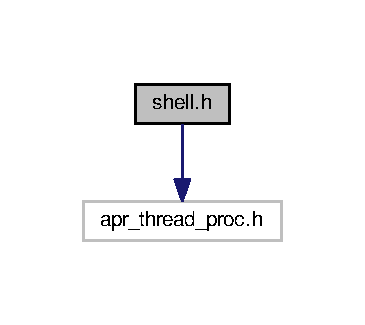
\includegraphics[width=175pt]{shell_8h__incl}
\end{center}
\end{figure}
This graph shows which files directly or indirectly include this file\+:\nopagebreak
\begin{figure}[H]
\begin{center}
\leavevmode
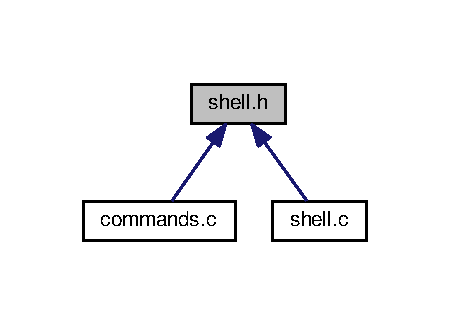
\includegraphics[width=216pt]{shell_8h__dep__incl}
\end{center}
\end{figure}
\subsection*{Classes}
\begin{DoxyCompactItemize}
\item 
struct \hyperlink{structShell}{Shell}
\end{DoxyCompactItemize}
\subsection*{Macros}
\begin{DoxyCompactItemize}
\item 
\hypertarget{shell_8h_a0ad0666a1726541270e5b2a3594f242c}{}\#define {\bfseries M\+A\+X\+\_\+\+C\+O\+M\+M\+A\+N\+D\+\_\+\+A\+R\+G\+S}~100\label{shell_8h_a0ad0666a1726541270e5b2a3594f242c}

\end{DoxyCompactItemize}
\subsection*{Typedefs}
\begin{DoxyCompactItemize}
\item 
\hypertarget{shell_8h_a5a458a7123d8cffb7cb2fce306bad661}{}typedef struct \hyperlink{structShell}{Shell} {\bfseries Shell}\label{shell_8h_a5a458a7123d8cffb7cb2fce306bad661}

\end{DoxyCompactItemize}
\subsection*{Functions}
\begin{DoxyCompactItemize}
\item 
int \hyperlink{shell_8h_acda27d63b5d5da99f9b12d52f376b006}{Shell\+\_\+run} (apr\+\_\+pool\+\_\+t $\ast$p, \hyperlink{structShell}{Shell} $\ast$cmd)
\begin{DoxyCompactList}\small\item\em shell run \end{DoxyCompactList}\item 
int \hyperlink{shell_8h_acd5077414441ce4297b163ccdba1c1d4}{Shell\+\_\+exec} (\hyperlink{structShell}{Shell} cmd,...)
\begin{DoxyCompactList}\small\item\em shell execute \end{DoxyCompactList}\end{DoxyCompactItemize}
\subsection*{Variables}
\begin{DoxyCompactItemize}
\item 
\hypertarget{shell_8h_ac8575ca18e0cd8a397ecf8703d0a1e2e}{}\hyperlink{structShell}{Shell} {\bfseries C\+L\+E\+A\+N\+U\+P\+\_\+\+S\+H}\label{shell_8h_ac8575ca18e0cd8a397ecf8703d0a1e2e}

\item 
\hypertarget{shell_8h_a16b33613717f72f8845944f362a8e92f}{}\hyperlink{structShell}{Shell} {\bfseries G\+I\+T\+\_\+\+S\+H}\label{shell_8h_a16b33613717f72f8845944f362a8e92f}

\item 
\hypertarget{shell_8h_ac58f37e9e100ffc67d216b23aeb70185}{}\hyperlink{structShell}{Shell} {\bfseries T\+A\+R\+\_\+\+G\+Z\+\_\+\+S\+H}\label{shell_8h_ac58f37e9e100ffc67d216b23aeb70185}

\item 
\hypertarget{shell_8h_aa0b669cfcbe7b7ba61c39ca7cfbc3b16}{}\hyperlink{structShell}{Shell} {\bfseries T\+A\+R\+\_\+\+B\+Z2\+\_\+\+S\+H}\label{shell_8h_aa0b669cfcbe7b7ba61c39ca7cfbc3b16}

\item 
\hypertarget{shell_8h_a346ec2013949bbb903b144afbea185a7}{}\hyperlink{structShell}{Shell} {\bfseries C\+U\+R\+L\+\_\+\+S\+H}\label{shell_8h_a346ec2013949bbb903b144afbea185a7}

\item 
\hypertarget{shell_8h_a0b00c62afcd9cbe9ddcafd077958746e}{}\hyperlink{structShell}{Shell} {\bfseries C\+O\+N\+F\+I\+G\+U\+R\+E\+\_\+\+S\+H}\label{shell_8h_a0b00c62afcd9cbe9ddcafd077958746e}

\item 
\hypertarget{shell_8h_a5b265c6270c71a773cc4af9e3ced813a}{}\hyperlink{structShell}{Shell} {\bfseries M\+A\+K\+E\+\_\+\+S\+H}\label{shell_8h_a5b265c6270c71a773cc4af9e3ced813a}

\item 
\hypertarget{shell_8h_a237379db14a3952deeb7e942a49e4e2b}{}\hyperlink{structShell}{Shell} {\bfseries I\+N\+S\+T\+A\+L\+L\+\_\+\+S\+H}\label{shell_8h_a237379db14a3952deeb7e942a49e4e2b}

\end{DoxyCompactItemize}


\subsection{Detailed Description}
shell header 

\begin{DoxyAuthor}{Author}
peter liu \href{mailto:peter.liu.work@gmail.com.tw}{\tt peter.\+liu.\+work@gmail.\+com.\+tw} 
\end{DoxyAuthor}
\begin{DoxyVersion}{Version}
0.\+0 
\end{DoxyVersion}
\begin{DoxyDate}{Date}
2016-\/04-\/10 
\end{DoxyDate}


\subsection{Function Documentation}
\hypertarget{shell_8h_acd5077414441ce4297b163ccdba1c1d4}{}\index{shell.\+h@{shell.\+h}!Shell\+\_\+exec@{Shell\+\_\+exec}}
\index{Shell\+\_\+exec@{Shell\+\_\+exec}!shell.\+h@{shell.\+h}}
\subsubsection[{Shell\+\_\+exec}]{\setlength{\rightskip}{0pt plus 5cm}int Shell\+\_\+exec (
\begin{DoxyParamCaption}
\item[{{\bf Shell}}]{template, }
\item[{}]{...}
\end{DoxyParamCaption}
)}\label{shell_8h_acd5077414441ce4297b163ccdba1c1d4}


shell execute 


\begin{DoxyParams}{Parameters}
{\em template} & shell command template \\
\hline
{\em ...} & shell command arguments\\
\hline
\end{DoxyParams}
\begin{DoxyReturn}{Returns}
{\bfseries 0}\+: execute finish successfully ~\newline
{\bfseries -\/1}\+: error 
\end{DoxyReturn}
\hypertarget{shell_8h_acda27d63b5d5da99f9b12d52f376b006}{}\index{shell.\+h@{shell.\+h}!Shell\+\_\+run@{Shell\+\_\+run}}
\index{Shell\+\_\+run@{Shell\+\_\+run}!shell.\+h@{shell.\+h}}
\subsubsection[{Shell\+\_\+run}]{\setlength{\rightskip}{0pt plus 5cm}int Shell\+\_\+run (
\begin{DoxyParamCaption}
\item[{apr\+\_\+pool\+\_\+t $\ast$}]{p, }
\item[{{\bf Shell} $\ast$}]{cmd}
\end{DoxyParamCaption}
)}\label{shell_8h_acda27d63b5d5da99f9b12d52f376b006}


shell run 


\begin{DoxyParams}{Parameters}
{\em p} & A\+P\+R pool \\
\hline
{\em cmd} & shell command\\
\hline
\end{DoxyParams}
\begin{DoxyReturn}{Returns}
{\bfseries 0}\+: run finish successfully ~\newline
{\bfseries -\/1}\+: error 
\end{DoxyReturn}

%--- End generated contents ---

% Index
\backmatter
\newpage
\phantomsection
\clearemptydoublepage
\addcontentsline{toc}{chapter}{Index}
\printindex

\end{document}
